\documentclass[11pt]{article}
\usepackage[margin=1in]{geometry}
\usepackage[T1]{fontenc}
\usepackage{mathptmx}
\usepackage{amsmath,amssymb,amsthm}
\usepackage{booktabs,tabularx,array}
\usepackage{tikz}
\usetikzlibrary{arrows.meta,positioning}
\usepackage{cite}
\usepackage[hidelinks]{hyperref}
\hypersetup{pdftitle={Causal Roster Certificates for Session-Separated Accountable Multisignatures under Asynchronous Churn},pdfauthor={Haoyi Zhang and Huaijin Ran},pdfsubject={Causal authorization semantics, session separation, and a key-prefixed BGLS realization for accountable multisignatures under asynchronous membership churn},pdfkeywords={accountable multisignatures, aggregate signatures, causal membership, key rotation, authorization certificates, partial orders, revocation, asynchronous systems}}
\newtheorem{theorem}{Theorem}[section]
\newtheorem{lemma}[theorem]{Lemma}
\newtheorem{proposition}[theorem]{Proposition}
\newtheorem{corollary}[theorem]{Corollary}
\theoremstyle{definition}
\newtheorem{definition}[theorem]{Definition}
\newtheorem{example}[theorem]{Example}
\newcommand{\Id}{\mathcal I}
\newcommand{\Act}{\operatorname{Act}}
\newcommand{\Max}{\operatorname{Max}}
\newcommand{\own}{\operatorname{own}}
\newcommand{\val}{\operatorname{val}}
\newcommand{\enc}{\operatorname{enc}}
\newcommand{\supp}{\operatorname{supp}}
\newcommand{\lo}{C_{\min}}
\newcommand{\hi}{C_{\max}}
\newcommand{\botkey}{\bot}
\allowdisplaybreaks
\title{Causal Roster Certificates for Session-Separated\\Accountable Multisignatures under Asynchronous Churn}
\author{Haoyi Zhang\\Xi'an Jiaotong-Liverpool University, Suzhou, China\\\texttt{hyeliozhang@gmail.com}\\ORCID: \texttt{0009-0009-3693-786X}
\and Huaijin Ran\\Nanyang Technological University, Singapore\\\texttt{huaijin003@e.ntu.edu.sg}}
\date{}
\begin{document}
\maketitle
\begin{abstract}
Accountable multisignatures identify the parties authorizing a common message, but a changing service must also identify the causal roster and exact key versions under which that authorization is valid. We model an authenticated membership history as a finite event poset and evaluate rosters at downward-closed cuts; concurrent maximal writes for one identity quarantine that identity. For a fixed signer/version profile and lower and upper view bounds, we prove that all authorizing cuts are either empty or one interval with explicit least and greatest endpoints. This yields exact historical, view-fresh, and window-robust tests. We then give a session-separated compiler: every selected long-term version key delegates to a fresh one-session base key while binding the complete causal context and identity--event--key table. A generic reduction decomposes completed framing into history, encoding, delegation, or one-session base failures. A linear executable reference profile uses an Ed25519-signed history checkpoint, Ed25519 delegations, and one exact-message signature per selected ephemeral key. Separately, key-prefixed Boneh--Gentry--Lynn--Shacham aggregation realizes a one-group-element proof-level base under its multi-user random-oracle theorem. Neither profile hides the linear table, delegations, signer description, or history evidence. Weighted roster selection is polynomial by maximum closure when each identity's writes form a chain, but NP-complete with quarantined forks even for unit weights and height-three histories. Cached authenticated views cannot reveal undisclosed revocations or certify complete observation.
\end{abstract}
\noindent\textbf{Keywords:} accountable multisignatures; aggregate signatures; causal membership; session separation; key rotation; authorization certificates; revocation; asynchronous systems.

\section{Introduction}\label{sec:intro}
An accountable multisignature answers a cryptographic question: which registered parties authorized a common message?  A service with asynchronous membership changes must answer a second question before that attribution is useful: \emph{which versions of those parties were jointly authorized when the message was signed?}  The two questions are not equivalent.  A valid contribution under Alice's previous key and one under Bob's current key may refer to states that cannot coexist in any causally consistent roster.  Conversely, an old roster may remain internally coherent and cryptographically authentic after a revocation has occurred at a replica that the verifier has not observed.

This distinction disappears when membership is idealized as a totally ordered sequence of epochs.  An epoch number silently assumes that every relevant join, removal, and rotation can be placed in one agreed order before authorization.  In an asynchronous execution, independently issued updates form only a partial order.  A verifier may know a lower causal floor that every admissible explanation must contain and an upper authenticated view beyond which it makes no completeness claim.  Between those bounds lie many cuts.  A completed aggregate should not be called authorized merely because every signer is current at \emph{some} cut; the selected versions must be current together at one cut or, under a stronger policy, at every cut compatible with the verifier's information.

Recent accountable multisignatures make the gap practically relevant.  Boneh, Partap, and Waters construct schemes with local key generation, constant-size stored public verification keys, and signatures whose cryptographic part is constant beyond the signer-set description~\cite{boneh2025accountable}.  Those properties address static key storage and signer accountability.  They do not by themselves assign temporal meaning to a mutable registration state.  Moreover, the most direct dynamic wrapper creates a second proof gap: if the same long-term signer key is placed in many changing registration tables, a theorem for one fixed table may not let a reduction answer signing queries in all the others.

\paragraph{The problem.}
We study a finite authenticated event history.  Every membership write names an identity, exact version, active or inactive status, long-term public key, weight, and declared causal parents.  Cuts are order ideals.  A unique visible maximal write determines an identity's state; incomparable maxima quarantine it until a later resolver dominates them.  Given ideals $L\subseteq U$ and an exact profile $Q$, we ask: (1) does some cut in $[L,U]_{\Id}$ authorize all entries simultaneously; (2) does every cut do so; and (3) how can a completed accountable multisignature bind the answer without assuming cross-table security for a reused long-term base key?

The first two questions are order-theoretic.  The third is a construction and reduction question.  A roster digest alone does not authenticate governance, prove a view complete, establish that an identity/version maps to the algebraic signer key, or upgrade a one-instance multisignature theorem to many mutable tables.  We therefore keep semantic, authentication, delegation, and base-multisignature obligations separate.

\paragraph{Exact causal authorization.}
For a fixed profile, all compatible cuts are either empty or form one interval $[C_{\min},C_{\max}]$ in the distributive lattice of ideals.  The lower endpoint is the downward closure of the verifier floor and selected versions.  The upper endpoint removes every later or incomparable same-owner write together with its descendants.  Possible authorization is exactly $C_{\min}\subseteq C_{\max}$; universal authorization is exactly $C_{\min}=L$ and $C_{\max}=U$.  Infeasibility always has a one- or two-entry profile obstruction, although validating it may traverse an arbitrarily long causal path.

The interval theorem gives three non-enumerative modes.  A historical certificate names one compatible cut.  A view-fresh certificate evaluates the upper view itself and rejects a selected version displaced or quarantined by a write already visible there.  A window-robust certificate requires validity at every cut between the bounds.  These modes form a strict hierarchy and are signed as distinct policies; changing a mode tag after signing is not allowed even when one predicate logically implies another.

\paragraph{Session-separated compiler.}
Our main construction treats each history event's public key as a long-term delegation key.  Once a semantic context and exact profile are fixed, every selected party generates a fresh accountable-multisignature key for that session.  The ordered ephemeral table is included in the canonical causal statement.  Each selected long-term version key signs a typed delegation binding its identity, exact event, ephemeral key, application message, session, namespace, history, bounds, mode, cut field, and full table.  After verifying the complete delegation vector, the parties run the base accountable multisignature once on that statement under the ephemeral table.

This arrangement has a deliberate cost and a deliberate benefit.  It adds one ephemeral public key and one ordinary delegation signature per selected identity, plus two setup broadcasts before the base protocol.  In return, an honest base secret occurs in only one registration table.  The generic reduction therefore uses a single-session exact-message attribution game and ordinary multi-user chosen-message security for delegations.  For at most $q_s$ honest session tables, completed framing advantage is bounded by the sum of history failure, context-binding failure, delegation forgery, and $q_s$ times the one-session base advantage.  We instantiate the full verification path with a central Ed25519-signed checkpoint, Ed25519 delegations, and a linear vector of one-session Ed25519 signatures.  We separately instantiate the compact aggregate layer with key-prefixed BGLS: the full ephemeral table and signer set are encoded in the common message, so a framed protected signer gives a multi-user aggregate forgery.  A direct wrapper using long-term keys remains possible, but it must separately prove the stronger joint multi-instance property.

The compiler preserves the useful meaning of constant persistent verification state when the history authenticator and component public parameters are constant-size.  It does not make the complete certificate constant: the profile, ephemeral table, delegation vector, and history evidence grow with the authorization.  This accounting prevents dynamic state from being hidden inside an uncounted ``public key'' or signer descriptor.

\paragraph{Boundaries and evidence.}
If every identity's writes form a chain, nonnegative weighted roster selection reduces to classical maximum closure~\cite{picard1976closure}.  With unresolved same-owner forks and quarantine, selection is NP-complete even for unit active weights and height-three histories, by a direct independent-set reduction~\cite{karp1972reducibility}.  Separately, no cached-view verifier can reject a remote revocation it has not received, and a signed parent list proves declared dependencies rather than every event a dishonest signer actually observed.

All general statements are proved in the article.  The artifact contains two finite implementations of the roster semantics, archived flow and hardness diagnostics, the strict V3 codec, and an end-to-end Ed25519 reference certificate with adversarial field-mutation tests.  The cryptographic tests establish only that the packaged implementation performs the stated parsing and public-key checks; they are not proofs of Ed25519 or of the general theorems.  The earlier finite-enumeration activity exceeded its cumulative ceiling before the accounting defect was found, and later reruns cannot restore compliance.  We therefore withdraw every computational-support claim for the mathematical results and rely on their written proofs.

The executable Ed25519 profile is intentionally linear and centralizes checkpoint issuance; it closes the parser-and-verifier path without claiming aggregation or decentralized governance.  The BGLS-KP realization is proof-level rather than a pairing implementation or benchmark.  It uses public-key prefixing, validation of every ephemeral key, and multi-user aggregate unforgeability in the random-oracle model.  Its aggregate is one group element, but its public-key table is linear.  Neither profile claims the constant registry-key compression of Boneh, Partap, and Waters; a theorem-level mapping for that stronger candidate remains separate.

\paragraph{Organization.}
Section~\ref{sec:related} positions the result.  Sections~\ref{sec:model} and~\ref{sec:windows} define the causal model and prove the interval theorem.  Section~\ref{sec:compiler} gives the modes and session-separated construction.  Section~\ref{sec:security} proves semantic soundness, attribution, stale-version rejection, and size accounting.  Section~\ref{sec:selection} gives the optimization and observation boundaries.  Section~\ref{sec:evidence} records proof status, the invalidated computational activity, and reproducibility limits.  Section~\ref{sec:conclusion} concludes.

\section{Background and related work}\label{sec:related}
The problem joins four bodies of work: multisignature accountability, dynamic public-key state, authenticated histories, and consistent-cut reasoning.  Each supplies a different obligation.  Signatures authenticate messages but do not choose a registration state; logs authenticate records but not signer intent; causal snapshots define coherent states but not the authenticity or completeness of their events.

\subsection{From multisignatures to accountable signer sets}
Early multisignatures distinguish joint authorization from independent signatures~\cite{itakura1983multisignatures}.  Signer-subset accountability makes participation explicit and forbids framing an honest nonparticipant~\cite{micali2001accountable}.  Pairing-based signatures then supplied compact algebraic components: Gap-Diffie--Hellman threshold and multisignature variants~\cite{boldyreva2003threshold}, BLS short signatures~\cite{boneh2001short}, and BGLS aggregation~\cite{boneh2003aggregate}.  None removes the need for a registration model or rogue-key defense.

Key prefixing is the closest bridge from aggregate unforgeability to exact signer attribution.  Lacharit\'e proves key-prefixed BGLS secure in a multi-user aggregate-forgery game that permits adversarial co-keys but requires one unqueried challenge-key/message pair in the accepted aggregate~\cite{lacharite2018multiuser}.  Current BLS implementation guidance uses the same augmentation pattern and requires nonidentity and subgroup validation~\cite{boneh2026blsdraft}; we use the peer-reviewed theorem for security and the draft only for validation syntax.  Encoding the immutable table and exact signer set in the common message makes this game fit our one-session failure, although the complete table remains linear.

Other registration defenses include the plain-public-key model and general forking lemma~\cite{bellare2006plain} and proofs of possession~\cite{ristenpart2007pop}.  Sequential and unrestricted aggregation order signature accumulation or messages~\cite{lu2006sequential,bellare2007aggregate,lysyanskaya2004sequential,brogle2012lazy,fischlin2012historyfree,gentry2018unified}; our partial order instead governs membership information.  Schnorr and BLS systems optimize fixed-universe storage, rounds, concurrency, and verification~\cite{boneh2018compact,maxwell2019musig,nick2021musig2,drijvers2019security,kojima2024tight,baldimtsi2024subset}.  They remain base-layer candidates only after their signer-set and registration games are matched to the causal statement.

The same separation applies beyond pairings.  Lattice multisignatures and aggregates cover two-round, quantum-random-oracle, synchronized, and online variants~\cite{damgard2021lattice,fukumitsu2020lattice,boschini2022musigl,elbansarkhani2014aggregate,fleischhacker2023chipmunk}; generic group-action work targets additional signature families~\cite{dalconzo2025groupaction}.  The compiler therefore asks only for exact-message attribution on one immutable table.  Its main cryptographic anchor, Boneh--Partap--Waters, instead provides accountable multisignatures with local key generation and constant stored verification state~\cite{boneh2025accountable}.  We add temporal semantics and avoid reusing one long-term base secret across changing tables; we do not reproduce that paper's registry compression.  Ordered composition, signer privacy, ad-hoc groups, compact compilers, traceable accountability, and standard-model aggregation improve orthogonal dimensions~\cite{baum2025ordered,haidar2025privacy,lehmann2024adhoc,jiang2025compact,wang2026traceable,hohenberger2025aggregate}.

\subsection{Threshold signatures and distributed setup as contrasts}
Threshold signatures authorize qualified subsets under one jointly controlled key; multisignatures retain separately generated keys and expose participation to the accountability mechanism.  Under churn, the former may refresh shares or rerun distributed key generation~\cite{gennaro1999dkg,canny2004dkg,groth2021dkg}, while the latter selects among independently registered versions.  FROST, adaptive Schnorr/BLS analyses, weighted qualification, and proactive refresh refine participation and compromise guarantees~\cite{komlo2021frost,crites2023adaptive,bacho2022threshold,baird2023multiverse,boneh2022proactive}.  A roster label alone supplies no erasure or forward security.

We consequently exclude abort blame and liveness.  Asynchronous broadcast and agreement establish communication or state consistency under explicit assumptions~\cite{cachin2001secure,cachin2000constantinople,reiter1996secure}; a signature equation does not imply those properties.  Conversely, an agreement protocol still needs a rule identifying which key versions were eligible.

\subsection{Dynamic membership, revocation, and key evolution}
Models for fully dynamic group signatures cover joins, leaves, tracing, anonymity, and revocation lists~\cite{bootle2020dynamic}.  Their opening-based goal differs from visible multisignature attribution, but their discipline transfers: key registration, corruption timing, and the moment a version becomes protected must be explicit.

Dynamic accumulators authenticate set membership or nonmembership, while verifier-side revocation moves work to the verifier~\cite{camenisch2002accumulator,nguyen2005accumulator,boneh2004vlr}.  They do not choose among incomparable writes for one identity; the accumulated statement still needs a concurrency policy.  Forward-secure and key-insulated signatures instead limit what secret compromise enables~\cite{bellare1999forward,itkis2001forward,dodis2002keyinsulated}.  Public authorization and secret evolution compose, but neither implies the other.  Our game therefore treats versions reusing one secret as one exposure domain.

Changing committees in systems such as Ouroboros Praos and Algorand motivate compact authorization under adaptive membership~\cite{david2018praos,gilad2017algorand}.  We do not analyze those protocols or inherit their synchrony and committee semantics.

\subsection{Causal histories and authenticated state}
Lamport's happened-before relation gives the partial-order language~\cite{lamport1978time}; consistent global states are order ideals.  Distributed snapshots, vector-style timestamps, virtual time, and dynamic interval clocks provide operational representations~\cite{chandy1985snapshots,fidge1988timestamps,mattern1989virtual,almeida2008itc}.  Our theorems use only the ideal abstraction and do not assume any clock is trustworthy.

CRDTs demonstrate that concurrent writes require an explicit merge policy~\cite{shapiro2011crdt,baquero2017pure}.  We quarantine incomparable maximal writes until a resolver dominates them, sacrificing availability rather than selecting by timestamp or identifier.  Other policies require new current-state predicates and new endpoint proofs.

Time-stamping, Merkle authentication, timeline entanglement, tamper-evident logs, transparency systems, and authenticated dictionaries can bind histories and views~\cite{haber1991timestamp,bayer1993timestamp,merkle1990certified,maniatis2002timeline,crosby2009logging,melara2015coniks,laurie2013ct,goodrich2008outsourced}.  They cannot prove that an unseen event does not exist.  Likewise, signed parent lists or signatures of knowledge bind declared relations but not everything a dishonest signer observed~\cite{chase2006knowledge}.  Our indistinguishability limits are local-view arguments, although Byzantine and asynchronous-consensus impossibilities provide broader context~\cite{dolev1982byzantine,fischer1985consensus}.

\subsection{Cuts, lattices, and optimization}
The ideals of a finite poset form a distributive lattice~\cite{birkhoff1937rings,davey2002lattices}, and distributed predicate detection searches such cuts without enumerating every state~\cite{garg1995predicate}.  Our fixed-profile predicate factors into lower requirements and upper exclusions, hence one interval; this is not a solver for arbitrary predicates.

With chain-ordered writes, weight differences reduce roster selection to maximum closure and one minimum cut~\cite{picard1976closure}.  Fork quarantine introduces conflicts; Section~\ref{sec:selection} embeds independent set~\cite{karp1972reducibility}.  Polynomial checking of one profile and polynomial optimization over all profiles are therefore distinct.

\subsection{Composition boundary}
Universal composability provides a stronger replacement discipline, including ordered multisignature functionalities~\cite{canetti2001uc,baum2025ordered}.  We prove a narrower game-based decomposition into history, encoding, delegation, and exact-message attribution failures.  The concrete paths are a linear Ed25519 profile~\cite{bernstein2012ed25519} and a proof-level BGLS-KP aggregate; ordinary signature unforgeability supplies the delegation premise~\cite{goldwasser1988digital}.  Persistent state, certificate growth, view completeness, and compromise timing remain separate claims.

\section{Authenticated event histories and roster cuts}\label{sec:model}
\subsection{The input history}
A history is a finite directed acyclic graph whose vertex set is $E$. Each event $e$ has a unique identifier, an owner $\own(e)$, a finite list of parents, and a membership value. The value is either inactive or an active public-key value with a nonnegative weight $w(e)$. The parent relation generates a reflexive partial order $\leq$: a parent precedes its child. Event identifiers name versions exactly. Two events may contain the same public-key bytes but still name different versions.

The history has already passed an external authentication and admission rule. This assumption includes the binding between an identity and its authorized membership writes. It is not discharged by checking that the graph is acyclic, parsing a key field, or computing a digest. The rule may admit two independently authorized writes that are concurrent. Thus authentication does not imply that the writes of one identity are totally ordered.

We call $\leq$ the \emph{declared order}. It records the dependencies carried by the input. An application wishing to interpret it as every event actually observed by a party needs an additional observation-completeness premise. Until Section~\ref{sec:observations}, every use of causality means the declared order, not physical time or an unrecorded local observation.

For $X\subseteq E$, define
\[
 \downarrow X=\{e\in E: e\leq x\text{ for some }x\in X\},\qquad
 \uparrow X=\{e\in E: x\leq e\text{ for some }x\in X\}.
\]
Reflexivity includes $X$ in both closures. The down-closure of the empty set is empty.

\begin{definition}[Causal cut]
A cut is an order ideal $C\subseteq E$: if $e\in C$ and $d\leq e$, then $d\in C$. Write $\Id(E)$ for the family of cuts. For cuts $L\subseteq U$, define
\[
 [L,U]_{\Id}=\{C\in\Id(E):L\subseteq C\subseteq U\}.
\]
\end{definition}

The two bounds have asymmetric roles. The lower bound is a floor that every admissible certificate must include, such as information already authenticated by a verifier. The upper bound is the portion of the finite history admitted to the query. It is not a statement that all real events have arrived. Both bounds must themselves be ideals; silently closing an invalid bound changes the question rather than validating it.

\subsection{A conservative policy for concurrent writes}
Let $E_i=\{e\in E:\own(e)=i\}$. For a cut $C$, consider the maximal elements of $E_i\cap C$ under $\leq$. The roster value for $i$ is active at event $e$ precisely when that maximal set is $\{e\}$ and the membership value written by $e$ is active. Let $\Act(C)$ be the resulting partial map from identities to active event identifiers.

This rule has three non-active outcomes: no visible write, a unique inactive maximal write, or several incomparable maximal writes. The last case is \emph{quarantine}. Quarantine is a chosen safety policy. Other applications may choose an add-wins, remove-wins, or total-order conflict rule, and the theorems below need not hold unchanged for them.

Quarantine is not irreversible. If two writes $x$ and $y$ are incomparable and a later write $z$ has both as ancestors, then a cut containing $z$ can have $z$ as its unique maximal write. The policy therefore recognizes an explicit resolving event rather than pretending that an arbitrary identifier ordering resolves causality.

\begin{definition}[Exact signer profile]
A profile $Q$ is a finite partial map from identities to event identifiers. It is authorized at $C$ when
\[
 \Act(C)(i)=Q(i)\qquad\text{for every }i\in\supp(Q).
\]
The profile need not include every active identity at $C$. It does include at most one version of each selected identity.
\end{definition}

Profiles containing an unknown event, an event of the wrong owner, or an inactive event are invalid. The empty profile is mathematically authorized at every cut. An aggregate-signature interface should reject it unless the application deliberately defines an empty authorization; the interface considered here rejects it.

\begin{figure}[t]
\centering
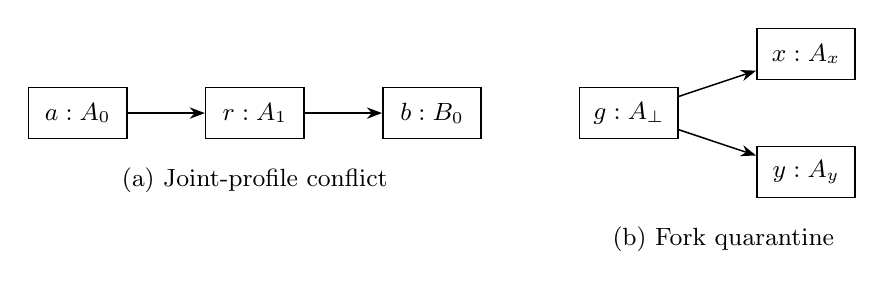
\begin{tikzpicture}[x=1cm,y=1cm,>=Stealth,
  event/.style={draw,rectangle,minimum width=1.25cm,minimum height=.65cm,inner sep=5pt,font=\small},
  every path/.style={line width=.55pt}]
\node[event] (a) at (0,0) {$a:A_0$};
\node[event] (r) at (2.25,0) {$r:A_1$};
\node[event] (b) at (4.5,0) {$b:B_0$};
\draw[->] (a)--(r);
\draw[->] (r)--(b);
\node[font=\small] at (2.25,-.85) {(a) Joint-profile conflict};
\node[event] (g) at (7,0) {$g:A_{\bot}$};
\node[event] (x) at (9.25,.75) {$x:A_x$};
\node[event] (y) at (9.25,-.75) {$y:A_y$};
\draw[->] (g)--(x);
\draw[->] (g)--(y);
\node[font=\small] at (8.2,-1.6) {(b) Fork quarantine};
\end{tikzpicture}

\caption{Declared-order constraints across and within identities. In (a), a cut containing Bob's event $b$ must contain Alice's rotation $r$, so the profile using $a$ and $b$ is impossible. In (b), a cut containing both $x$ and $y$ quarantines identity $A$; neither incomparable write is an authorized current version. An arrow runs from a declared parent to its child.}
\label{fig:conflicts}
\end{figure}

\subsection{Views, weights, and key exposure}
The active weight of a cut is
\[
 W(C)=\sum_{i\in\operatorname{dom}(\Act(C))}w\bigl(\Act(C)(i)\bigr).
\]
An inactive event contributes no weight even if a representation has a nonzero auxiliary weight field. Only the current active event matters. The optimization problem asks for $\max_{C\in[L,U]_{\Id}}W(C)$, not for the weight of an arbitrarily chosen set of events.

The event model does not treat corruption as a membership update. Exposure concerns the secret corresponding to a public-key value; authorization concerns an event and a cut. If two event versions reuse the same secret key, corrupting that secret exposes both versions. Calling one version ``old'' does not restore secrecy. Section~\ref{sec:security} therefore defines protection at the secret-key level and makes no forward-security claim from event labels alone.

\subsection{What the available view certifies}
A valid history establishes that its admitted events and dependencies can be checked according to the assumed governance rule. A valid cut establishes downward closure in that history. Authorization then establishes a relation between that cut and a specified profile. None of these statements identifies an observer-independent newest cut.

This separation also prevents a circular use of cryptography. An implementation cannot define an authorized history as ``the history accepted by the proposed scheme'' and then use that definition as a proof that the scheme rejects unauthorized events. Authentication and admission must have their own explicit mechanism or be a stated input assumption. They remain input assumptions throughout the finite implementation in this note.

\section{The exact interval for a fixed signer profile}\label{sec:windows}
\subsection{A local characterization with global consequences}
The meaning of a unique current write has a simple order-theoretic form. Finiteness matters: a nonempty subset of a finite poset has a maximal element above each of its elements.

\begin{lemma}[Unique-maximum characterization]\label{lem:maximum}
Let $e$ be an active write owned by $i$. For a cut $C$, the equality $\Act(C)(i)=e$ holds if and only if $e\in C$ and every write in $E_i\cap C$ is at most $e$.
\end{lemma}
\begin{proof}
If $e$ is the unique maximal element, begin at any $x\in E_i\cap C$ and repeatedly move to a strictly larger element of that set while possible. Since the set is finite, the process stops at a maximal element, necessarily $e$. Hence $x\leq e$. Conversely, if $e\in C$ and every element of $E_i\cap C$ is at most $e$, then $e$ is its greatest element and therefore its unique maximal element. Its active value supplies the required roster entry.
\end{proof}

For an active profile $Q$ whose chosen events all lie in $U$, define the set of forbidden writes
\begin{equation}\label{eq:bad}
 B_Q=\bigcup_{i\in\supp(Q)}\{x\in E_i\cap U:x\not\leq Q(i)\}.
\end{equation}
This includes both later writes and incomparable writes for a chosen identity. A forbidden write also forbids all its descendants from a compatible ideal. Define
\begin{equation}\label{eq:endpoints}
 \lo=\downarrow\bigl(L\cup\{Q(i):i\in\supp(Q)\}\bigr),\qquad
 \hi=U\setminus\uparrow B_Q.
\end{equation}
The closure in the first formula is taken in $E$; because $U$ is an ideal containing its generators, it remains inside $U$. The up-closure in the second formula may be taken in $E$ and intersected with $U$, or directly in $U$.

\begin{theorem}[Exact authorization window]\label{thm:window}
Let $L\subseteq U$ be cuts of a finite history, and let $Q$ be a profile. If a chosen event is unknown, inactive, belongs to a different identity, or lies outside $U$, there is no compatible cut. Otherwise compute~\eqref{eq:bad} and~\eqref{eq:endpoints}. Then
\begin{equation}\label{eq:family}
 \{C\in[L,U]_{\Id}:Q\text{ is authorized at }C\}
 =
 \begin{cases}
 [\lo,\hi]_{\Id},&\lo\subseteq\hi,\\
 \varnothing,&\text{otherwise}.
 \end{cases}
\end{equation}
In the nonempty case, $\lo$ and $\hi$ are respectively the unique least and greatest compatible cuts.
\end{theorem}
\begin{proof}
The preliminary invalid cases follow directly from the definition of authorization. Assume they do not occur. The set $\lo$ is an ideal by construction. To see that $\hi$ is an ideal, take $y\in\hi$ and $x\leq y$. Since $U$ is an ideal, $x\in U$. If $x\notin\hi$, a forbidden write $b\in B_Q$ satisfies $b\leq x\leq y$, contrary to $y\in\hi$. Thus $x\in\hi$.

Suppose $C$ is compatible. It contains $L$ and every chosen event, so downward closure gives $\lo\subseteq C$. By Lemma~\ref{lem:maximum}, $C$ contains no member of $B_Q$. If it contained a descendant of a forbidden write, downward closure would force that write into $C$. Hence $C\subseteq\hi$. These inclusions prove necessity and show that $\lo\not\subseteq\hi$ makes compatibility impossible.

For sufficiency, let $C$ be an ideal between $\lo$ and $\hi$. It contains every $Q(i)$. Consider any same-owner write $x\in E_i\cap C$. Because $C\subseteq U$ and $C$ excludes $B_Q$, the definition of $B_Q$ gives $x\leq Q(i)$. Lemma~\ref{lem:maximum} now gives $\Act(C)(i)=Q(i)$ for each selected identity. The floor and upper bound follow from $L\subseteq\lo$ and $\hi\subseteq U$. Finally, the two endpoints themselves are ideals and lie in the compatible family whenever they are nested, proving their extremal and uniqueness properties.
\end{proof}

The theorem checks the entire profile together. In the running example, $Q(A)=a$ and $Q(B)=b$. The forced closure contains $r$ because $r<b$, while $r\in B_Q$ because it is a write of $A$ above $a$. Consequently $r\in\lo\setminus\hi$. The rejected profile comes with a concrete causal inconsistency, not with evidence that either signer failed to produce a signature.

\subsection{Possible authorization is not universal authorization}
The exact family makes the two quantifiers explicit:
\[
 \operatorname{Possible}(L,U,Q)\iff\lo\subseteq\hi,
\]
where preliminary invalid profiles are assigned false, whereas
\[
 \operatorname{Universal}(L,U,Q)
 \iff \forall C\in[L,U]_{\Id},\ Q\text{ is authorized at }C.
\]
The underlying interval is nonempty, since it always contains $L$ and $U$.

\begin{corollary}[Universal authorization]\label{cor:universal}
For a valid active profile, universal authorization holds exactly when $\lo=L$ and $\hi=U$. Equivalently, every chosen version belongs to $L$ and every same-owner write in $U$ is at most that version.
\end{corollary}
\begin{proof}
If the two endpoints equal the view bounds, Theorem~\ref{thm:window} identifies the compatible family with the entire interval. Conversely, universality makes both $L$ and $U$ compatible. Extremality of the compatible endpoints gives $\lo\subseteq L$ and $U\subseteq\hi$, while the opposite inclusions always hold. Thus equality follows. The alternate formulation is obtained by substituting into~\eqref{eq:bad} and~\eqref{eq:endpoints}: $\lo=L$ means all chosen events already lie in the ideal $L$, and $\hi=U$ means $B_Q$ is empty.
\end{proof}

For example, an old version can be possible in $[\varnothing,U]_{\Id}$ even though $U$ contains its rotation. It cannot be universal there. More generally, a nonempty profile is never universal when the lower bound is empty, because the empty cut authorizes no identity. This is not a failure of the theorem: it identifies how strong the universal claim is.

If a verifier advances its floor from $L$ to $L'$ with $L\subseteq L'\subseteq U$, possible authorization can disappear but cannot appear. Indeed the query family only shrinks. The lower endpoint becomes the closure of $L'$ with the selected versions; the upper endpoint is unchanged for fixed $U$ and $Q$. By contrast, enlarging only the upper view preserves any old authorizing cut, although it may invalidate freshness at the new upper cut or robustness over the enlarged interval. Changing both bounds combines these effects and has no unconditional direction.

\subsection{Pairwise compatibility and small obstructions}
Individually feasible signers are insufficient. Pairwise compatibility, however, is enough under this policy. This consequence describes an obstruction in the \emph{profile}, not a constant-size cryptographic proof about the entire history.

\begin{proposition}[Two-profile obstruction]\label{prop:helly}
For each chosen active event $e$, let $\mathcal F_e$ be its compatible-cut family in the common interval $[L,U]_{\Id}$. A finite collection of chosen events has a common compatible cut if and only if every singleton family is nonempty and every pair of families intersects. Consequently, an infeasible profile has an infeasible subprofile of size at most two.
\end{proposition}
\begin{proof}
Necessity is immediate. For sufficiency, write each nonempty family as $[a_e,b_e]_{\Id}$ using Theorem~\ref{thm:window}. Pairwise intersection implies $a_e\subseteq b_f$ for all $e,f$; the diagonal case follows from singleton feasibility. Thus
\[
 A=\bigcup_e a_e\ \subseteq\ \bigcap_f b_f=B.
\]
A union and an intersection of ideals are ideals, so $A$ belongs to every $[a_e,b_e]_{\Id}$. It is a common compatible cut. Taking the contrapositive proves the obstruction bound. Distinct versions of the same identity have disjoint families, so allowing such a collection does not evade the argument.
\end{proof}

The proposition does not say that two events are all the evidence a verifier needs. An incompatibility may involve a long dependency path, and certifying the absence of an order relation can require consulting the supplied history. Nor does the obstruction identify a malicious party. Two honest signers can select individually valid versions from incompatible views. The statement concerns joint authorization, not culpability.


\subsection{View-extension laws}
The endpoint formulas also show how the three acceptance modes react when a verifier learns more.  These laws are useful for cache design because they distinguish a claim that is invariant under a larger upper view from one that must be re-evaluated.

\begin{proposition}[Monotonicity under view refinement]\label{prop:viewlaws}
Fix a history $E$, a profile $Q$, and ideals $L\subseteq U\subseteq U'$ such that every selected event lies in $U$.
\begin{enumerate}
  \item $\operatorname{Possible}(L,U,Q)$ holds if and only if $\operatorname{Possible}(L,U',Q)$ holds.
  \item If $Q$ is authorized at $U'$, then it is authorized at $U$.  The converse can fail.
  \item If $Q$ is universal on $[L,U']_{\Id}$, then it is universal on $[L,U]_{\Id}$.  If $L\subseteq L'\subseteq U$ and $Q$ is universal on $[L,U]_{\Id}$, then it is universal on $[L',U]_{\Id}$.
  \item If $\operatorname{Possible}(L',U,Q)$ holds for $L\subseteq L'\subseteq U$, then $\operatorname{Possible}(L,U,Q)$ holds.  The converse can fail.
\end{enumerate}
\end{proposition}
\begin{proof}
For the forward direction of item~1, an authorizing cut inside $U$ remains a cut inside $U'$.  For the reverse direction, let $C'\in[L,U']_{\Id}$ authorize $Q$ and put $C=C'\cap U$.  Intersections of ideals are ideals, $C$ contains $L$ and every selected event, and $C\subseteq U$.  Removing events cannot introduce a same-owner write that is later than or incomparable with a selected unique maximum.  Hence $Q$ remains authorized at $C$.

For item~2, if a selected event $e$ is the unique maximal write of its owner in $U'$, every same-owner write in $U'$ is at most $e$ by Lemma~\ref{lem:maximum}; the statement remains true in the subset $U$.  The converse fails when $U'$ adds a later or incomparable same-owner write.  The first implication of item~3 follows because $[L,U]_{\Id}$ is a subfamily of $[L,U']_{\Id}$; the second follows because $[L',U]_{\Id}$ is a subfamily of $[L,U]_{\Id}$.  Item~4 follows from the inclusion of cut families.  A stronger floor can force a write that conflicts with a selected version, so the reverse implication need not hold.
\end{proof}

Possible historical authorization is therefore stable once the floor, profile, and the selected events are fixed: enlarging only the upper view cannot create or destroy the existence of some earlier compatible cut.  What changes is the range of admissible explanations and the stronger modes.  View-fresh and robust certificates must be rechecked whenever $U$ advances; a historical certificate can be retained for audit, provided its explicit cut and the verifier's current floor are still acceptable under application policy.

\subsection{Concise semantic failure certificates}
The endpoint computation gives more than a Boolean answer.  An invalid profile entry is witnessed by the entry itself and the authenticated event record.  For a well-formed active profile, infeasibility has a short causal explanation.

\begin{proposition}[Path witness for profile infeasibility]\label{prop:path-witness}
Assume all entries of $Q$ are admitted active writes of the correct owners and lie in $U$.  If $Q$ is infeasible in $[L,U]_{\Id}$, then one of the following witnesses exists.
\begin{enumerate}
  \item A \emph{floor witness} $(e,b)$, where $e=Q(i)$, $b\in E_i\cap U$, $b\not\leq e$, and $b\leq z$ for some $z\in L$.
  \item A \emph{pair witness} $(e,f,b)$, where $e=Q(i)$, $f=Q(j)$ for $i\neq j$, $b\in E_i\cap U$, $b\not\leq e$, and $b\leq f$.
\end{enumerate}
Conversely, either witness proves infeasibility.  The order relations can be certified by parent paths in the authenticated history.
\end{proposition}
\begin{proof}
Infeasibility means $\lo\nsubseteq\hi$.  Choose $y\in\lo\setminus\hi$.  Because $y\notin\hi=U\setminus\uparrow B_Q$, there is $b\in B_Q$ with $b\leq y$.  Because $y$ lies in the downward closure of $L$ and the selected events, there is a generator $z\in L\cup\{Q(j):j\in\supp(Q)\}$ with $y\leq z$.  Thus $b\leq z$.  By definition of $B_Q$, $b$ is a write of some selected identity $i$ and $b\not\leq e=Q(i)$.

If $z\in L$, the first witness results.  Otherwise $z=f=Q(j)$.  We cannot have $j=i$, because then $b\leq f=e$ would contradict $b\not\leq e$; hence $i\neq j$ and the second witness results.

For the converse, any compatible cut contains $L$ and every selected event.  Downward closure therefore forces $b$ into the cut from either $z\in L$ or $f$.  Since the same cut must contain $e$ and $b\not\leq e$, Lemma~\ref{lem:maximum} says that $e$ cannot be the unique current write of its owner.  Thus no compatible cut exists.
\end{proof}

A verifier need not trust a claimed transitive-closure matrix to check this witness.  It can validate one parent path from $b$ to $z$ and separately establish that $b\not\leq e$ by recomputing reachability in the authenticated finite view.  The positive path is succinct; the non-reachability check is generally global unless the history authenticator supplies a sound nonmembership or non-ancestry proof.

Robust-mode failure has an even simpler description.  If $\lo\neq L$, some selected event is absent from $L$.  If $\hi\neq U$, there is a forbidden same-owner write in $U$.  These two cases are exactly the two clauses of Corollary~\ref{cor:universal}.  They make policy diagnostics intelligible: a robust certificate fails either because the lower view has not yet established a selected version or because the upper view already contains a competing version.

\subsection{Computation and certificates}
An elementary implementation computes the transitive predecessor sets in topological order, unions the forced sets, marks forbidden writes, and removes their descendants. A direct graph-search implementation uses $O(n(n+m))$ time and $O(n^2)$ reachability bits for $n$ vertices and $m$ parent edges, after which the endpoint computation is polynomial in $n$ and the profile size. Packed bitsets reduce constants; they must not be treated as unit-cost words when $n$ grows without bound.

The endpoint pair is a compact \emph{semantic} summary once the authenticated history is available. A separate verifier can reconstruct both endpoints or enumerate all cuts in a small model and check that the same family is obtained. Neither method authenticates the input history. The executable study uses both a bitset implementation and a set-based exhaustive oracle, while Proposition~\ref{prop:helly} is supported by its general proof rather than a separate finite experiment.

\section{Causal-roster certificates and session separation}\label{sec:compiler}
The interval theorem determines whether a profile is authorized in a declared history.  A completed cryptographic authorization must bind that statement to the message and to the exact signer evidence.  We first define three temporal acceptance modes, then give a session-separated compiler that turns long-term version keys into one-session exact-set signing keys.  The separation is the construction-level step that removes a hidden cross-table assumption: no honest base signing key is reused when the roster changes.  The compiler is generic; Section~\ref{sec:security} also instantiates its base interface with key-prefixed BGLS aggregation.

\subsection{Long-term and session-local primitives}
The compiler uses three independently specified components.

\paragraph{Authenticated history.}
A history-authentication interface has public parameters $pp_H$, a persistent verification key $vk_H$, and an algorithm
\[
  \mathsf{HistVerify}(pp_H,vk_H,\mathsf{tag},\mathsf{ns},\Gamma,L,U,\pi_H)\in\{0,1\}.
\]
The tag $\mathsf{tag}$ and namespace $\mathsf{ns}$ separate protocol and membership domains.  Acceptance means that $\Gamma,L,U$, including owner, key, status, weight, and parent fields, were admitted by the external governance rule and that event identifiers are unambiguous.  A signed checkpoint, transparency proof, or authenticated dictionary may realize the interface; acyclicity alone is insufficient.

\paragraph{Version-key delegation signatures.}
Each active event $e$ carries a long-term digital-signature verification key $dpk(e)$.  Its secret key signs only typed delegation statements defined below.  The signature scheme $\mathsf{DS}=(\mathsf{DGen},\mathsf{DSign},\mathsf{DVerify})$ must be secure against adaptive chosen-message attacks in the multi-user setting.  Reusing one $dpk$ in several versions of the same identity creates one exposure domain.  Registering the same $dpk$ for different identities is rejected by governance, because otherwise a valid delegation could be relabelled without a forgery.

\paragraph{One-session accountable multisignature.}
For one immutable session table $P=(epk_1,\ldots,epk_k)$, the base scheme supplies local key generation, its registration or proof-of-possession procedure, partial signing, aggregation, and public verification.  We write
\[
  \mathsf{BVerify}(K_P,\mu,S_P,\sigma)=1
\]
when the completed signature is valid for common message $\mu$ and signer-index set $S_P$ under the verification object $K_P$ derived from $P$.  The exact base transcript may be interactive; only its completed output enters the certificate.  Section~\ref{sec:security} requires exact-message attribution for one such table, including the base scheme's actual rogue-key model.  It first proves a generic composition theorem and then shows that BGLS-KP realizes the interface when $K_P$ is the validated ordered table and the exact table and signer set are encoded into the signed message.  Unlike the direct-key baseline discussed below, the main compiler never places a long-term version key in two base tables.

\subsection{Canonical semantic commitment}
Let $pp=(pp_H,\enc,H,\mathsf{ids})$ fix the history parameters, encoding, hash, and algorithm/type identifiers; $\mathsf{tag}$ is instead an explicit certificate field signed at both layers.  The encoding $\enc$ is injective, prefix-free, and type-separated: integers use fixed endianness and lengths, sets and maps are sorted, an event includes its namespace, identity, owner, status, key, weight, and ordered parents, a cut lists sorted event identifiers, and a profile lists sorted triples $(i,e,dpk(e))$.

Let $H$ be collision resistant and domain separated.  We use
\[
 h_\Gamma=H(\mathsf{hist}\parallel\enc(\Gamma)),\quad
 h_L=H(\mathsf{cutL}\parallel\enc(L)),\quad
 h_U=H(\mathsf{cutU}\parallel\enc(U)),
\]
with analogous digests $h_C$ and $h_Q$.  Using full encodings would remove the hash-collision event at the price of a larger message.  In either case, the verifier needs the encoded data or a sound proof of the relevant predicate.  A short digest does not prove view completeness, downward closure, or freshness.

The context fields $(\mathsf{tag},\mathsf{app},\mathsf{sid},m)$ map respectively to \texttt{domain}, \texttt{application}, \texttt{session}, and \texttt{message} in the executable profile.  Session uniqueness is an application invariant, not a clock epoch, and replay remains an application-state question.

\subsection{Acceptance modes}
The same history can support three different temporal claims.  Treating them as one Boolean predicate would hide the policy choice.

\begin{definition}[Historical mode $\mathsf{HIST}$]
A historical claim contains a cut $C$.  It is semantically valid for $(L,U,Q)$ when $C\in[L,U]_{\Id}$ and $Q$ is authorized at $C$.
\end{definition}
Historical mode says that the selected versions coexist at one authenticated causal state that includes the verifier's floor.  It does not claim that the versions are current at the upper view.  This mode is appropriate for auditing an authorization whose time is represented by the named cut.

\begin{definition}[View-fresh mode $\mathsf{FRESH}$]
A view-fresh claim is semantically valid for $(L,U,Q)$ when $Q$ is authorized at $U$.
\end{definition}
Because $U$ is the newest state within the verifier's admitted view, this mode rejects any selected version displaced or quarantined by a write already visible in $U$.  It remains view-relative: an unseen remote revocation is outside the statement.

\begin{definition}[Window-robust mode $\mathsf{ROBUST}$]
A window-robust claim is semantically valid for $(L,U,Q)$ when $Q$ is authorized at every $C\in[L,U]_{\Id}$.
\end{definition}
By Corollary~\ref{cor:universal}, robust mode holds exactly when the profile's compatible interval equals the entire view interval.  Every selected event must already be in $L$, and $U$ may contain no same-owner write that is later than or incomparable with a selected version.  Robustness is therefore much stronger than existence of one historical cut.


\begin{proposition}[Strict hierarchy of temporal claims]\label{prop:modes}
For fixed $(L,U,Q)$,
\[
  \mathsf{ROBUST}\Longrightarrow\mathsf{FRESH}\Longrightarrow\mathsf{HIST}.
\]
Both implications are strict in general.
\end{proposition}
\begin{proof}
Robustness quantifies over every cut in $[L,U]_{\Id}$ and therefore includes $U$, proving the first implication.  If $Q$ is authorized at $U$, historical mode can choose $C=U$, proving the second.

For strictness of the second implication, let $e<r$ be two writes of one identity, with $e$ and $r$ active, take $L=\varnothing$, $U=\{e,r\}$, and select $e$.  The cut $\{e\}$ establishes historical validity, while $e$ is not current at $U$.  For strictness of the first, take one active event $e$, $L=\varnothing$, $U=\{e\}$, and select $e$.  The profile is fresh at $U$ but cannot be robust because the empty cut in the interval does not contain $e$.
\end{proof}

The hierarchy is semantic, not a license to rewrite certificates.  Because the mode tag is included in $\mu$, a signature produced for $\mathsf{ROBUST}$ does not verify after an aggregator changes the tag to $\mathsf{FRESH}$, even though the underlying predicate implies it.  This choice prevents a verifier from being shown one policy while signers approved another.  An application that wants one signature to satisfy several policies can define a fourth, explicitly signed policy whose verification rule returns the strongest proved status and lets the application accept weaker consequences without mutating the context.

The three modes also lead to different cache rules.  A historical certificate should retain the exact cut $C$ and the history evidence needed to validate it; later upper-view extensions do not invalidate the existence of that cut, although a stronger local floor may make the application reject it.  A view-fresh certificate is a statement about a particular $U$ and should be re-evaluated or replaced when the accepted checkpoint advances.  A robust certificate is stable under strengthening the lower floor inside the same $U$, but can fail when $U$ expands with a competing same-owner write.  Proposition~\ref{prop:viewlaws} makes these rules precise.

\begin{table}[t]
\centering
\caption{Interpretation of the three signed modes.  ``Newest'' is always relative to the admitted upper view, never to undisclosed global events.}
\label{tab:modes}
\begin{tabularx}{\linewidth}{@{}p{.17\linewidth}p{.24\linewidth}X@{}}
\toprule
Mode & Semantic question & Typical use and invalidation condition\\
\midrule
$\mathsf{HIST}$ & Does one named cut authorize the exact profile? & Archival or delayed execution; fails if the cut or profile is invalid, or if a verifier policy requires a stronger floor not contained in the cut.\\
$\mathsf{FRESH}$ & Does the upper view itself authorize the profile? & Online use at one checkpoint; fails when that view contains a later or incomparable same-owner write.\\
$\mathsf{ROBUST}$ & Do all cuts between the bounds authorize the profile? & Authorization insensitive to uncertainty inside a view window; fails if a selected event is absent from the floor or a competing write appears in the upper view.\\
\bottomrule
\end{tabularx}
\end{table}

\subsection{The session-separated compiler}\label{subsec:session-compiler}
Let $Q=((i_1,e_1),\ldots,(i_k,e_k))$ be the canonically ordered exact profile.  After the semantic context and mode predicate are fixed, every selected signer generates a fresh base key pair $(esk_j,epk_j)$ for this session and publishes $epk_j$ together with whatever registration evidence the base scheme requires.  The canonical ephemeral table is
\[
 P=((i_1,e_1,epk_1),\ldots,(i_k,e_k,epk_k)).
\]
The verifier rejects a missing entry, a duplicate identity, a duplicate ephemeral public key, or an entry whose identity/event pair is not exactly the corresponding member of $Q$.  Honest signers never reuse $esk_j$ in another session.

For each mode define the distinguished cut field
\[
 C^*=\begin{cases}
 C,&\mathsf{mode}=\mathsf{HIST},\\
 U,&\mathsf{mode}=\mathsf{FRESH},\\
 \bot,&\mathsf{mode}=\mathsf{ROBUST}.
 \end{cases}
\]
The bottom symbol is a typed constant, not an omitted byte string.  Define the common session statement
\begin{align}
 \chi=\enc(&\mathsf{CAUSAL\mbox{-}ROSTER\mbox{-}SESSION\mbox{-}V3},
 \mathsf{tag},\mathsf{mode},\mathsf{app},\mathsf{sid},m,\mathsf{ns},h_\Gamma,h_L,h_U,\nonumber\\
 &H(\mathsf{cutC}\parallel\enc(C^*)),h_Q,P).
 \label{eq:session-statement}
\end{align}
Signer $i_j$ issues the long-term delegation
\begin{equation}
 \delta_j=\mathsf{DSign}_{dsk(e_j)}
   (\enc(\mathsf{DELEGATE\mbox{-}V3},\chi,i_j,e_j,epk_j)).
 \label{eq:delegation}
\end{equation}
The common base message is
\begin{equation}
 \mu=\enc(\mathsf{BASE\mbox{-}AMS\mbox{-}V3},\chi,Q,P,S_P),
 \qquad S_P=\{1,\ldots,k\}.
 \label{eq:context}
\end{equation}
The redundant occurrence of $Q$ and $P$ in $\mu$ makes the executable profile self-describing after parsing; injective encoding would remain sufficient if they were referenced only through $\chi$.  It is unnecessary to hash the signature bytes $\delta_j$ into $\mu$: every accepted delegation verifies over the same $\chi$ and its unique table entry.  Binding the randomized signature encodings would add an extra synchronization round without changing the authorized statement.

The pre-protocol has two ordered broadcasts before the ordinary base protocol.  First, all ephemeral public keys and registration evidence are collected and the full table $P$ is frozen.  Second, each selected version key signs its delegation only after validating the complete semantic context and $P$; all honest participants check the full delegation vector.  They then run the base accountable multisignature on the exact $\mu$.  If the base protocol is itself interactive, these are setup broadcasts in addition to its rounds.  A party that has not seen the final $P$ or the final semantic statement must not delegate or base-sign.

A certificate is
\[
 \tau=(\mathsf{tag},\mathsf{mode},\mathsf{app},\mathsf{sid},m,\mathsf{ns},\Gamma,\pi_H,
 L,U,C^*,Q,P,\Delta,K_P,\sigma),
\]
where $\Delta=(\delta_1,\ldots,\delta_k)$.  A deployment may replace explicit history data by content-addressed objects and sound proofs.  The logical fields remain part of the signed statement even when transmitted out of band.

\begin{definition}[Certificate verification]
Given public parameters $pp$, persistent history key $vk_H$, and certificate $\tau$, the verifier performs the following checks.
\begin{enumerate}
  \item Parse every field under one canonical encoding and reject duplicate identities, duplicate events, malformed keys, an empty profile, or an unknown mode.
  \item Verify $\mathsf{HistVerify}(pp_H,vk_H,\mathsf{tag},\mathsf{ns},\Gamma,L,U,\pi_H)$ and reconstruct the declared partial order.  Check that $L,U$ are ideals and $L\subseteq U$.
  \item Check every profile entry is an admitted active write of the named identity, lies in $U$, and contains the long-term delegation key used below.
  \item For $\mathsf{HIST}$, require $C^*\in[L,U]_{\Id}$ and authorization of $Q$ there.  For $\mathsf{FRESH}$, require $C^*=U$ and authorization at $U$.  For $\mathsf{ROBUST}$, require $C^*=\bot$ and $C_{\min}=L$, $C_{\max}=U$ by Theorem~\ref{thm:window}.
  \item Check that $P$ is the exact, duplicate-free table for $Q$ and validate the base scheme's registration evidence.  Recompute $\chi$.
  \item For every $(i_j,e_j,epk_j)$, verify $\delta_j$ under $dpk(e_j)$ on the typed delegation message in~\eqref{eq:delegation}.
  \item Derive or recompute $K_P$, reconstruct $\mu$ and $S_P$, and accept only if $\mathsf{BVerify}(K_P,\mu,S_P,\sigma)=1$.
\end{enumerate}
\end{definition}
The order gives logical dependencies, not a side-channel prescription.  The pair $(pp,\tau)$ reconstructs every history, delegation, and base payload, including $\mathsf{tag}$; a valid aggregate cannot excuse malformed history or reuse a delegation for another table.

\subsection{Correctness and direct-key baseline}
Correctness follows from deterministic reconstruction.  If the history proof is honest, the selected mode predicate holds, every signer receives the same canonical context and table, all delegations verify, and the base protocol completes correctly on $\mu$, certificate verification accepts.  No synchrony or completion guarantee follows: parties may fail to collect one common view, table, delegation vector, or base transcript.

A simpler direct-key wrapper can place the long-term version keys themselves in the base table.  Its certificate is smaller because it omits $P$ and $\Delta$, but the same honest base key then appears across many tables as unrelated members join or rotate.  Security no longer follows from a one-table attribution theorem.  It needs a joint multi-instance theorem that answers signing queries for the same challenge key across every admissible table, or a construction-specific reduction proving that property.  The session-separated compiler pays linear delegation evidence and fresh key generation precisely to avoid that premise.

The running conflict $a<r<b$ illustrates both layers.  The profile $\{A\mapsto a,B\mapsto b\}$ cannot reach the cryptographic phase because no cut authorizes it.  The singleton $\{A\mapsto a\}$ may enter historical mode before $r$, but not fresh mode once $r\in U$.  If it enters, Alice's long-term key at event $a$ delegates only to the fresh $epk_A$ inside that exact historical statement; neither a later session nor a different table can reuse the delegation.

\subsection{Persistent state and transmitted evidence}
Table~\ref{tab:sizes} separates persistent state from per-authorization communication.
\begin{table}[t]
\centering
\caption{Objects in the session-separated certificate.  ``Constant'' means bounded by the security parameter independently of identities and events.}
\label{tab:sizes}
\begin{tabularx}{\linewidth}{@{}p{.25\linewidth}X@{}}
\toprule
Object & Role and size qualification\\
\midrule
$vk_H$ and public parameters & Persistent trust anchor and algorithm parameters; constant only for the instantiated history, delegation, and base schemes.\\
$Q$ & Exact identity/version description; information content grows with the selected set.\\
$P,\Delta$ & One ephemeral base key and one long-term delegation signature per selected identity; linear unless a separately proved compression mechanism is added.\\
$\Gamma,L,U,C^*,\pi_H$ & History and view evidence; explicit transmission grows with events, while succinct proofs need their own soundness and update analysis.\\
$K_P,\sigma$ & Session verification object and completed base aggregate.  In the BGLS-KP realization, $K_P=P$ is linear while $\sigma$ is one source-group element.\\
Application replay state & Optional state keyed by $(\mathsf{app},\mathsf{sid})$; not part of public-key size.\\
\bottomrule
\end{tabularx}
\end{table}

A $b$-bit descriptor cannot independently identify all $k$-subsets of an $n$-identity universe unless $2^b\geq\binom nk$.  This observation is not a lower bound on persistent verification state because the signer set may be supplied separately.  It does explain why constant-size base signatures do not make the complete causal certificate constant-size.  Session separation leaves the base aggregate compact when the base scheme does, but adds $k$ ephemeral keys and $k$ delegations.

\subsection{What the compiler does not provide}
The compiler binds signers to a precise causal statement and removes long-term base-key reuse.  The BGLS-KP realization closes one compact aggregate interface.  Section~\ref{subsec:ed25519-reference} also gives a central signed-checkpoint and linear Ed25519 reference profile for executable end-to-end verification; neither profile supplies decentralized governance or global freshness.  They do not prove global freshness beyond $U$, give forward security after secret compromise, prove completeness of a signer's observations, ensure liveness, prevent replay of an identical certificate, hide the signer set, or attribute an aborted ceremony.  Nor does the BGLS result turn an unrelated base theorem with incompatible registration or signer-set semantics into the single-session game.  Those are separate construction or systems obligations.

\section{Security definitions and composition}\label{sec:security}
This section proves the main construction theorem.  Session separation replaces the previous cross-table premise by two standard-looking obligations: chosen-message security for long-term delegation signatures and exact-message accountability for one freshly generated base table.  The theorem remains conditional on the concrete schemes satisfying the games actually stated here; it does not infer those games from an abstract interface name.

\subsection{Adversarial model and protected entries}
The adversary controls message delivery, may present different admitted upper views to different sessions, registers malicious base keys as permitted by the base scheme, obtains honest delegations and base-signing interactions, and exposes secrets.  Governance decides which history records are admitted; an invalid record can pass only through history-authentication failure.

A version entry $(i,e)$ is protected in a session only while both its long-term delegation secret $dsk(e)$ and its fresh session secret $esk_{i,e,\mathsf{sid}}$ remain unexposed.  Reusing a long-term key in several same-owner versions creates one long-term exposure domain.  Honest ephemeral secrets are generated independently for one table and are never reused.  Rotation changes which public key is authorized; it does not imply erasure or retrospective protection.

For certificate $\tau$, let
\[
 \mathsf{Sess}(\tau)=(\chi,P,K_P,\mu,S_P)
\]
be the exact tuple reconstructed from Equations~\eqref{eq:session-statement}--\eqref{eq:context}.  An honest wrapper authorization for entry $(i,e)$ records both the exact delegation message and honest base participation on this tuple.  Recording only application message $m$ is insufficient because the same message can occur under different histories, bounds, modes, profiles, tables, and sessions.

\subsection{Component games}
\paragraph{History soundness.}
For fixed $pp$, protocol tag, namespace, and governance rule, the adversary wins if it produces $(\mathsf{tag},\mathsf{ns},\Gamma,L,U,\pi_H)$ accepted by $\mathsf{HistVerify}(pp_H,vk_H,\mathsf{tag},\mathsf{ns},\Gamma,L,U,\pi_H)$ although a parsed field or bound was not admitted.  Let $\epsilon_H$ bound this probability.  Sound authentication of a received view is not proof that no undisclosed event exists.

\paragraph{Context binding.}
The adversary wins if two distinct interpreted session statements accepted by the canonical parser produce the same $\chi$ or if two distinct base contexts produce the same $\mu$.  Complete injective encoding gives zero advantage.  With digests for large fields, a win yields an encoding ambiguity or hash collision.  Let the resulting bound be $\epsilon_B$.

\paragraph{Multi-user delegation unforgeability.}
The delegation challenger generates polynomially many long-term signature keys and answers adaptive signing and corruption queries.  A forgery is an accepted signature under an unexposed key on a typed delegation message never signed under that key.  The message includes $\chi$, identity, exact event, and ephemeral public key.  Let $\epsilon_D$ bound the adversary's multi-user chosen-message advantage.  This is the usual role of adaptive signature security~\cite{goldwasser1988digital}, specialized only by domain separation.

\paragraph{Single-session exact-message attribution.}
The base challenger creates one immutable table $P$ containing any number of protected honest ephemeral keys and adversarially registered keys under the base scheme's real registration model.  It answers honest signing interactions on exact tuples $(K_P,\mu,S)$ and records, for every protected key, the tuple on which participation was supplied.  The adversary wins by outputting an accepted $(K_P,\mu,S,\sigma)$ that includes an unexposed protected key for which no honest participation was recorded on that exact tuple.  Let $\epsilon_A$ bound this one-table advantage.

The signer set belongs to the authorization record.  A definition that records only $\mu$ is insufficient when a partial contribution for one set can be reused in another.  Encoding $S$ into $\mu$ is necessary, but the base theorem must also cover the actual interactive transcript and aggregation rule.  The game permits malicious co-signers and keys because the compiler does not assume every selected party is honest.

\subsection{Wrapper accountability game}
The wrapper challenger provides $(pp,vk_H)$ and access to honest session creation.  A request fixes a parseable semantic context through $Q$.  The challenger checks the same history and temporal predicate as the public verifier.  For each selected protected entry it generates a fresh base key pair, freezes $P$, returns the exact delegation on $\chi$, and exposes the base signing interface only for $(K_P,\mu,S_P)$.  Invalid contexts receive no honest authorization.  Corruption of either relevant secret removes that entry/session from the protected set.

The adversary wins if it outputs an accepted certificate $\tau$ and protected entry $(i,e)$ for which the challenger did not record both the exact delegation and exact base participation in $\mathsf{Sess}(\tau)$.  The game concerns a completed accepted authorization.  It does not blame silence, a malformed partial contribution, or an aborted interaction.

\begin{theorem}[Semantic soundness]\label{thm:semantic-soundness}
Assume no history-soundness failure and canonical parsing.  Every accepted certificate satisfies the semantic predicate of its encoded mode.  Its ephemeral table contains exactly one distinct base key for every exact profile entry, and every such key is delegated by the long-term public key stored in that entry.
\end{theorem}
\begin{proof}
History soundness fixes the admitted events, owner bindings, long-term keys, and declared order.  The verifier checks that $L,U$ are ideals, $L\subseteq U$, and each selected entry is an active write for its claimed owner.  Historical and fresh acceptance are their definitions.  Robust acceptance follows from endpoint equality and Corollary~\ref{cor:universal}, without enumeration.

Canonical table checks give one identity/event/ephemeral-key tuple per profile entry and reject aliases.  Each accepted delegation verifies under the exact $dpk(e)$ authenticated in that event on a message containing the same $\chi$, identity, event, and ephemeral key.  Hence no accepted table entry is substituted for another without a history, parsing, or signature failure.
\end{proof}

\begin{theorem}[Session-separated exact-message attribution]\label{thm:composition}
Let a wrapper adversary activate at most $q_s\geq1$ honest session tables.  There are component adversaries of comparable running time such that
\[
 \operatorname{Adv}^{\mathsf{ss\mbox{-}attr}}
 \leq \epsilon_H+\epsilon_B+\epsilon_D+q_s\epsilon_A.
 \label{eq:security-bound}
\]
The reduction preserves history, corruption, delegation, and signing queries up to deterministic wrapper checks.  No independence assumption among bad events is used.
\end{theorem}
\begin{proof}
Let $B_H$ and $B_B$ denote history and context-binding failures.  Their union has probability at most $\epsilon_H+\epsilon_B$.  Condition on their complement and on an accepted winning certificate $\tau$ framing protected $(i,e)$.

The verifier accepted a delegation $\delta_i$ under the authenticated long-term key $dpk(e)$ on the exact typed message $(\chi,i,e,epk_i)$.  If the challenger never issued this delegation, the same output is a multi-user chosen-message forgery, contributing at most $\epsilon_D$.  Otherwise, an honest request fixed exactly the interpreted semantic context and ephemeral table in $\tau$: absence of $B_B$ prevents another context from sharing $\chi$.

Because the wrapper output is nevertheless winning, the protected ephemeral key $epk_i$ did not receive honest base participation on the exact $(K_P,\mu,S_P)$ accepted in $\tau$.  The key is unexposed and appears in no other honest session table.  A base reduction guesses uniformly one of the at most $q_s$ honest tables, embeds its one-table challenge there, and generates all other session keys itself.  When the guessed table is the framed one, the accepted $\sigma$ is an exact-message attribution forgery in the single-session game.  Thus the conditioned wrapper success probability is at most $q_s\epsilon_A$.  Adding the three earlier failure probabilities proves~\eqref{eq:security-bound}.
\end{proof}

The $q_s$ factor is explicit rather than hidden in the phrase ``multi-user security.''  A construction-specific base proof can improve it by giving a tight multi-instance theorem.  The compiler's point is more basic: simulation of non-target sessions is possible because their honest base keys are freshly generated by the reduction, not long-lived challenge keys reused across mutable roster tables.


\subsection{Executable signed-checkpoint and Ed25519-vector profile}\label{subsec:ed25519-reference}
The generic theorem can be exercised end to end without implementing a pairing by using a deliberately noncompact reference profile.  It is not the efficiency construction: its completed base evidence contains one ordinary signature per selected entry.  Its value is narrower.  It fixes an executable history authenticator, delegation scheme, codec, and exact-message base verifier, so every logical field in the compiler can be checked by real public-key verification rather than byte-string equality.

Let $(hsk,hpk)$ be an Ed25519 key pair~\cite{bernstein2012ed25519}.  For a declared view define
\[
 \eta_H=\enc(\mathsf{CAUSAL\mbox{-}ROSTER\mbox{-}HISTORY\mbox{-}V1},
        \mathsf{tag},\mathsf{ns},\Gamma,L,U).
\]
A central checkpoint issuer returns $\pi_H=\mathsf{EdSign}_{hsk}(\eta_H)$ only after its external admission rule accepts the explicit protocol domain, namespace, events, key fields, parent edges, and bounds.  The corresponding history verifier checks this signature under the persistent $hpk$.  This profile authenticates exactly the received view; it does not prove that the issuer is honest, that all replicas have converged, or that no later event exists.

Every active event carries an Ed25519 delegation key.  The typed message is exactly Equation~\eqref{eq:delegation}, with the full identity--event--ephemeral-key triple and session statement.  Each ephemeral key is also Ed25519.  Instead of aggregating, entry $j$ returns
\[
   \rho_j=\mathsf{EdSign}_{esk_j}(\mu),
   \qquad
   \sigma_{\mathsf{vec}}=((i_1,e_1,epk_1,\rho_1),\ldots,
                          (i_k,e_k,epk_k,\rho_k)).
\]
The base verifier requires this ordered vector to match $P$ exactly, rejects missing, extra, duplicate, or reordered entries under the canonical syntax, and verifies every $\rho_j$ on the same $\mu$.  The vector therefore gives transparent exact-set attribution but has $\Theta(k)$ signature size; it is a baseline, not an aggregate-signature claim.

\begin{theorem}[Conditional security of the executable profile]\label{thm:ed25519-reference}
Assume an injective canonical encoding, that the checkpoint issuer signs only admitted history payloads, and EUF-CMA security of Ed25519 under independently generated keys.  Let $q_D$ bound the number of protected long-term delegation keys that can witness a wrapper forgery, and let $k_{\max}$ bound one session table.  Then the reference profile realizes the component games with
\[
 \epsilon_H\leq \operatorname{Adv}^{\mathsf{EUF\mbox{-}CMA}}_{\mathsf{Ed25519},H},\qquad
 \epsilon_D\leq q_D\operatorname{Adv}^{\mathsf{EUF\mbox{-}CMA}}_{\mathsf{Ed25519},D},
\]
and
\[
 \epsilon_A\leq k_{\max}
 \operatorname{Adv}^{\mathsf{EUF\mbox{-}CMA}}_{\mathsf{Ed25519},E}.
\]
The factors may be replaced by the corresponding multi-user advantages when the assumed games supply all challenge keys and the wrapper's adaptive non-target corruptions.
\end{theorem}
\begin{proof}
An accepted unadmitted view contains a valid checkpoint signature on an $\eta_H$ that the correct issuer did not sign, unless two interpreted views have the same encoding.  This gives the first reduction.  For delegations, guess the unexposed long-term key that witnesses the final violation, embed the EUF-CMA challenge there, generate every other key locally, answer its signing queries through the oracle, and answer non-target corruption queries directly.  Conditioned on the guess, an accepted unissued typed delegation is a forgery; guessing loses at most $q_D$.

The base reduction is identical at session scale.  Guess the protected ephemeral entry that will witness the violation, embed the challenge key there, and generate every other ephemeral key locally.  Exact participation queries for the guessed entry are signing-oracle queries on $\mu$; non-target signing and exposure queries are answered directly.  If the guess is the final unexposed framed entry, the accepted vector contains a valid signature on an unqueried $\mu$.  The loss is at most $k_{\max}$.  A matching multi-user game can remove these target guesses directly.
\end{proof}

\begin{corollary}[Reference-profile wrapper bound]\label{cor:ed25519-composition}
For at most $q_s$ session tables and at most $k_{\max}$ selected entries per table,
\[
 \operatorname{Adv}^{\mathsf{ss\mbox{-}attr}}
 \leq \operatorname{Adv}^{\mathsf{EUF\mbox{-}CMA}}_{\mathsf{Ed25519},H}
      +\epsilon_B
      +q_D\operatorname{Adv}^{\mathsf{EUF\mbox{-}CMA}}_{\mathsf{Ed25519},D}
      +q_s k_{\max}\operatorname{Adv}^{\mathsf{EUF\mbox{-}CMA}}_{\mathsf{Ed25519},E}.
\]
\end{corollary}
\begin{proof}
Substitute Theorem~\ref{thm:ed25519-reference} into Theorem~\ref{thm:composition}.
\end{proof}

The corollary is a linear-size end-to-end profile.  Its \texttt{domain} field realizes $\mathsf{tag}$ in $\eta_H$, $\chi$, and $\tau$; identifiers are bounded printable US-ASCII, while messages admit Unicode scalars but not surrogate code points, making the ASCII-escaped encoding injective on the admitted domain.  Before use, every active event key, selected or not, must decode as a canonical nonidentity prime-order Ed25519 point.  The verifier also rejects noncanonical bytes, cross-identity or cross-role aliases, duplicate or misbound entries, invalid signatures, and invalid roster semantics.  Same-owner key reuse remains event-bound.

This executable profile narrows, but does not erase, the deployment boundary.  The deterministic keys in the public example are test fixtures and are unusable as secrets.  The implementation delegates arithmetic and constant-time details to a maintained cryptographic library, does not prove that library correct, and supplies no key-storage, randomness, rollback, replay-database, or checkpoint-governance service.  Most importantly, the profile is linear and does not establish the compact aggregate or constant registry-key properties sought from the BGLS and accountable-multisignature layers.

\subsection{A concrete key-prefixed BGLS realization}\label{subsec:bgls-realization}
We now close the base interface with a named construction.  This realization is intentionally different from the compact-registry schemes that motivate the paper: it gives a one-group-element aggregate but sends the complete ephemeral public-key table.  Its purpose is to discharge the exact one-session attribution premise without hiding a stronger key-compression claim.

Let $(\mathbb G_1,\mathbb G_2,\mathbb G_T,p,e,g_1,g_2)$ be asymmetric bilinear-group parameters of prime order $p$, and let $H_B:\{0,1\}^*\rightarrow\mathbb G_1$ be a domain-separated random oracle.  For session entry $j$, sample $x_j\leftarrow\mathbb Z_p^*$ and publish
\[
 epk_j=(X_{1,j},X_{2,j})=(g_1^{x_j},g_2^{x_j}).
\]
Validation rejects identity elements, elements outside the prime-order subgroups, inconsistent pairs for which
$e(X_{1,j},g_2)\neq e(g_1,X_{2,j})$, and duplicate encoded keys.  These checks are part of $\mathsf{BVerify}$, not optional preprocessing.  They are the two-group analogue of the nonidentity and subgroup checks required by current BLS implementation guidance~\cite{boneh2026blsdraft}.

For an exact base tuple $(P,\mu,S)$ define
\begin{equation}
 \nu=\enc(\mathsf{BGLS\mbox{-}KP\mbox{-}CRS\mbox{-}V1},P,\mu,S).
 \label{eq:bgls-message}
\end{equation}
Signer $j\in S$ outputs
\[
 \sigma_j=H_B(\enc(\mathsf{BGLS\mbox{-}KP\mbox{-}SIG\mbox{-}V1},epk_j,\nu))^{x_j}\in\mathbb G_1,
\]
and aggregation multiplies the contributions, $\sigma=\prod_{j\in S}\sigma_j$.  After validating the table, the signer-index set, and $\sigma$, verification accepts exactly when
\begin{equation}
 e(\sigma,g_2)=\prod_{j\in S}
 e\!\left(H_B(\enc(\mathsf{BGLS\mbox{-}KP\mbox{-}SIG\mbox{-}V1},epk_j,\nu)),X_{2,j}\right).
 \label{eq:bgls-verify}
\end{equation}
Thus $K_P=P$.  Public-key prefixing makes the enhanced messages signer-specific even though all signers authorize the same $\nu$.  Encoding $P$, $\mu$, and $S$ inside $\nu$ additionally prevents a contribution authorized for one table or signer set from being transplanted into another.

Lacharit\'e's multi-user aggregate-unforgeability game gives the adversary challenge keys, permits adversarially generated co-keys, and declares a forgery nontrivial when one included challenge key/message pair was never submitted to its signing oracle.  For BGLS-KP, that paper proves a random-oracle reduction to multi-user BLS-KP and records the resulting reduction chain to the usual BLS assumptions~\cite{lacharite2018multiuser}.  This is exactly the malicious-co-key condition needed below; the current Internet-Draft is cited only for encoding and validation practice, not as the proof source.

\begin{theorem}[BGLS-KP realizes one-session exact attribution]\label{thm:bgls-base}
Assume injective encodings, the validation rules above, and the random-oracle model.  Let one base table contain at most $k_{\max}$ honest ephemeral keys, with entries removed from protection after exposure.  For every adversary against the single-session exact-message attribution game there is a BGLS-KP MU-A-EUF-CMA adversary of comparable running time such that
\[
 \epsilon_A\leq k_{\max}\,
 \operatorname{Adv}^{\mathsf{MU\mbox{-}A\mbox{-}EUF\mbox{-}CMA}}_{\mathsf{BGLS\mbox{-}KP}}.
 \label{eq:bgls-base-bound}
\]
If the base game forbids exposure of honest session secrets after table creation, the factor $k_{\max}$ is unnecessary.
\end{theorem}
\begin{proof}
The reduction guesses one honest table position that will witness the final violation.  It embeds a challenge BGLS-KP public key at that position, generates all other honest keys locally, and forwards any adversarially registered co-keys unchanged after validation.  A protected signing interaction on exact tuple $(P,\mu,S)$ becomes a signing-oracle query for the challenge key on the enhanced message determined by~\eqref{eq:bgls-message}; locally generated entries are answered directly.  Corruptions of locally generated entries are answered, while corruption of the guessed challenge entry causes an abort.  Because the wrapper counts only unexposed entries as protected, conditioning on guessing the framed entry avoids that abort.

Suppose the base adversary outputs an accepted $(P,\mu,S,\sigma)$ framing the guessed key.  The accepted pairing equation is a valid BGLS-KP aggregate.  Exact encoding of $P$, $\mu$, and $S$ implies that the corresponding challenge key/message pair was never queried: any query with another table, signer set, context, or session produces a different $\nu$.  The remaining aggregate keys may be challenge keys, locally generated keys, or adversarial keys, as allowed by MU-A-EUF-CMA.  Hence the output is a nontrivial multi-user aggregate forgery.  Guessing the framed honest position loses at most $k_{\max}$; without exposure queries all honest positions may be supplied as challenge keys and no position guess is needed.
\end{proof}

\begin{corollary}[Concrete wrapper bound]\label{cor:bgls-composition}
For BGLS-KP as the base scheme and sessions of at most $k_{\max}$ selected entries,
\[
 \operatorname{Adv}^{\mathsf{ss\mbox{-}attr}}
 \leq \epsilon_H+\epsilon_B+\epsilon_D
 +q_s k_{\max}\,
 \operatorname{Adv}^{\mathsf{MU\mbox{-}A\mbox{-}EUF\mbox{-}CMA}}_{\mathsf{BGLS\mbox{-}KP}}.
\]
Under the no-session-secret-exposure restriction, delete $k_{\max}$.
\end{corollary}
\begin{proof}
Substitute Theorem~\ref{thm:bgls-base} into Theorem~\ref{thm:composition}.
\end{proof}

The concrete aggregate $\sigma$ is one element of $\mathbb G_1$, while $P$ contains two group elements per signer in the proof-aligned syntax above.  A one-public-key-element implementation profile may be used only after its exact security theorem and validation rules are mapped to the same game.  No pairing timings, curve choice, byte counts, side-channel properties, or deployment security are claimed here.

\begin{proposition}[Why direct long-term use needs a stronger game]\label{prop:direct-key}
If an honest long-term version key is used directly as a base key in two different registration tables, a theorem for one fixed table does not by itself imply wrapper attribution across those tables.
\end{proposition}
\begin{proof}
A reduction embedding its challenge key in one table must still answer honest signing queries involving the same unknown secret in the other table.  A one-table challenger need not provide such an oracle.  Session separation removes the simulation request because the challenge secret belongs to one freshly generated table; alternatively, a direct construction must prove a joint multi-instance theorem that supplies or simulates the missing queries.
\end{proof}

\subsection{Freshness and stale-version rejection}
\begin{theorem}[View-relative stale-key rejection]\label{thm:stale}
Assume no history-soundness failure.  Let $(i,e)$ be selected and let $x\in E_i\cap U$ satisfy $x\not\leq e$.
\begin{enumerate}
  \item No $\mathsf{FRESH}$ certificate selecting $e$ is accepted for upper view $U$.
  \item No $\mathsf{ROBUST}$ certificate selecting $e$ is accepted for $[L,U]_{\Id}$.
  \item A $\mathsf{HIST}$ certificate may be accepted only at a cut excluding $x$ and every descendant of $x$.
\end{enumerate}
\end{theorem}
\begin{proof}
The event $x$ belongs to the forbidden set $B_Q$ of~\eqref{eq:bad}.  Fresh mode evaluates $U$, where Lemma~\ref{lem:maximum} rules out $e$ as the unique current write.  Robust mode implies authorization at $U$ and also fails.  Historical compatibility requires $C\subseteq C_{\max}=U\setminus\uparrow B_Q$, so $C$ excludes $x$ and its descendants.
\end{proof}
The statement is relative to the admitted upper view.  A deployment needing stronger freshness must require a fresh authority response, quorum checkpoint, age bound, or synchrony assumption and bind that evidence into $\chi$.  Section~\ref{sec:selection} proves that a cached view cannot reveal an undisclosed remote revocation.

\subsection{Persistent-key and certificate accounting}
\begin{theorem}[Conditional persistent-state inheritance]\label{thm:keysize}
Suppose the history authenticator has persistent verification-key length $c_H(\lambda)$ and the delegation and base schemes have public-parameter lengths $c_D(\lambda)$ and $c_A(\lambda)$, each independent of identities, versions, and sessions.  Then the session-separated verifier can retain persistent public cryptographic state of length
\[
 c_H(\lambda)+c_D(\lambda)+c_A(\lambda)+O(1).
\]
The certificate additionally contains $\Theta(|Q|)$ delegation keys/signatures unless a separate compression theorem applies.
\end{theorem}
\begin{proof}
Persistent state consists of the history trust anchor, fixed algorithm parameters, domain tags, and identifiers.  Long-term version public keys are authenticated fields of the supplied history, while the fresh table, delegations, session verification object, profile, bounds, and completed signature are supplied with the certificate.  Their sizes do not enter retained state.  Conversely, one distinct ephemeral key and one verified delegation are present for every selected profile entry, giving the stated linear certificate component under the uncompressed syntax.
\end{proof}
The theorem does not imply constant update bandwidth, proof-refresh cost, verification time, or total certificate size.  It preserves the useful persistent-state meaning of compact accountable multisignatures while making the session-separation cost visible.

\subsection{Corruption, replay, and instantiation boundary}
A rotation from $e$ to $e'$ changes the public delegation key authorized by fresh semantics.  Protection of past authorizations additionally depends on compromise timing, erasure, forward-secure signatures, or key insulation~\cite{bellare1999forward,itkis2001forward,dodis2002keyinsulated}.  The game treats an exposed long-term or session secret as unprotected; the compiler does not infer erasure from history.

Context binding prevents a certificate for one history, cut, mode, profile, session, or ephemeral table from verifying as another.  It does not prevent replay of the identical byte string.  Replay control is application state keyed by $(\mathsf{app},\mathsf{sid})$.  The theorem also does not prove that every signer received all events in the world; it proves only that protected signers authorized the exact authenticated view encoded in $\chi$.

The Ed25519 profile closes one central, linear implementation path but assumes correct checkpoint issuance and the stated signature-security games.  The BGLS-KP realization closes the compact one-session aggregate interface under the random-oracle and pairing assumptions above.  A deployment using it still must authenticate governance and declared parent edges, implement its canonical codec, instantiate a multi-user secure delegation signature, enforce fresh nonreused session keys, and select validated pairing parameters.  Boneh, Partap, and Waters provide stronger compact-registry functionality and local key generation, making their construction an attractive efficiency candidate~\cite{boneh2025accountable}.  This article does not claim a theorem-level mapping from their published game to ours; in particular, the BGLS-KP corollary does not inherit their constant stored public-key compression.

\subsection{Construction-level audit checklist}\label{subsec:audit-checklist}
Table~\ref{tab:audit} contrasts the wrappers and locates the remaining construction-specific proof obligations.

\begin{table}[t]
\centering
\caption{Direct-key and session-separated wrappers.  Neither supplies history authentication or global freshness.}
\label{tab:audit}
\begin{tabularx}{\linewidth}{@{}>{\raggedright\arraybackslash}p{.21\linewidth}>{\raggedright\arraybackslash}X>{\raggedright\arraybackslash}X@{}}
\toprule
Dimension & Direct long-term-key wrapper & Session-separated wrapper\\
\midrule
Base-key lifetime & Same version secret may occur in many changing tables & Each honest base secret belongs to one immutable table\\
Required base theorem & Joint multi-instance attribution across tables using a challenge key & Exact-message attribution for one table, with a session guess\\
Long-term authorization & Implicit in use of the version key as a base key & Typed delegation under the authenticated version key\\
Certificate growth & Omits ephemeral keys and delegations & One ephemeral key and delegation per selected identity\\
Reduction failure mode & Simulator may need the unknown secret in a non-target table & Non-target tables are generated locally\\
\bottomrule
\end{tabularx}
\end{table}

An audit of an alternative base has five checkpoints.  The BGLS-KP construction above meets the first two by explicit encoding and its cited malicious-co-key game.  First, the verification object must bind exactly one immutable $P$ and model the real proof-of-possession or malicious-key rule.  Second, the base game must bind the same $K_P$, canonical $\mu$, $S_P$, and transcript data relevant to reuse.  Third, its timing must cover the wrapper's malicious registrations, adaptive delegations, view choices, corruptions, and setup assumptions; a selective theorem cannot simply be renamed adaptive.

Fourth, implementations must enforce one fresh session key per frozen table.  Deterministic derivation needs domain-separated uniqueness and pseudorandomness; erasure may strengthen compromise resilience but is not assumed.  Fifth, compressing $P$, $\Delta$, or history evidence needs a separate binding or soundness theorem.  A failed checkpoint blocks that alternative named instantiation, not the generic compiler theorem or the BGLS-KP corollary proved above.

\section{Selection complexity and temporal limits}\label{sec:selection}\label{sec:optimization}
The exact-window algorithm evaluates one supplied profile.  Applications may instead optimize over all profiles or demand freshness beyond a declared view.  These are strictly harder questions.  The first half of this section separates a polynomial chain case from an NP-complete fork case.  The second half proves two information limits that no signature equation can remove.
The preceding section fixes the attributed signer versions. Sometimes an application instead asks how much active weight can coexist in some admissible cut. This is a selection problem over rosters, not merely an authorization check for a supplied profile. The distinction explains why a polynomial fixed-profile test does not imply a polynomial algorithm for the best profile.

\subsection{Per-identity chains and telescoping weights}
Assume first that every $E_i$ is a chain. Let $p_i(e)$ be the immediately preceding write of $i$ before $e$, when it exists, and define
\[
 v(e)=\begin{cases}w(e),&e\text{ active},\\0,&e\text{ inactive},\end{cases}
 \qquad
 \delta(e)=v(e)-\begin{cases}v(p_i(e)),&p_i(e)\text{ exists},\\0,&\text{otherwise}.\end{cases}
\]
A rotation may have negative $\delta$ even though all active weights are nonnegative. Negative increments are essential: ignoring them would retain retired weight in the objective.

\begin{lemma}[Telescoping identity weights]\label{lem:telescope}
For every ideal $C$ in a per-identity-chain history,
\begin{equation}\label{eq:telescope}
 W(C)=\sum_{e\in C}\delta(e).
\end{equation}
\end{lemma}
\begin{proof}
For each identity, $E_i\cap C$ is an initial segment of the chain $E_i$, since $C$ contains all predecessors of every included write. The sum of successive differences on this segment is zero if the segment is empty and otherwise equals the value of its last event. A nonempty segment has that event as its unique maximal write. Its value is therefore exactly the contribution of identity $i$ to $W(C)$. Summing over identities proves~\eqref{eq:telescope}.
\end{proof}

\subsection{A classical closure network with explicit bounds}
Let $D=\sum_{e\in E}|\delta(e)|$ and $M=D+1$. Form a directed network with source $s$, sink $t$, and one vertex for each event. Positive increments produce an arc $s\to e$ of capacity $\delta(e)$; negative increments produce an arc $e\to t$ of capacity $-\delta(e)$. For every declared parent edge $p\to e$, add the reversed arc $e\to p$ of capacity $M$. Force the floor by adding capacity $M$ on $s\to e$ for each $e\in L$, and exclude vertices outside $U$ by adding capacity $M$ on $e\to t$ for each $e\notin U$. Parallel capacities are summed.

Write $P_+=\sum_e\max(\delta(e),0)$. This is the maximum-closure reduction specialized to a bounded roster query, not a new flow algorithm~\cite{picard1976closure}. The finite capacity $M$ removes any need for an informal ``infinite'' number in the implementation or certificate.

\begin{theorem}[Exact chain optimization]\label{thm:closure}
If the writes of each identity form a chain, a minimum cut in the network above has source-side event set $C^*\in[L,U]_{\Id}$ and
\begin{equation}\label{eq:optimum}
 \max_{C\in[L,U]_{\Id}}W(C)=P_+-\operatorname{mincut}.
\end{equation}
The problem is polynomial-time solvable. A feasible flow and an admissible cut of equal flow/cut value certify the optimum without trusting the optimizer.
\end{theorem}
\begin{proof}
Consider the network cut with source side $\{s\}\cup L$. Since $L$ is an ideal and lies in $U$, no forcing or dependency arc crosses from that side to the sink side. Its capacity is at most $D<M$, being a sum of some positive and negative increment magnitudes. Thus a minimum cut cannot cut any arc of capacity at least $M$.

Let $C$ be the event set on the source side of a minimum cut. Avoiding reversed dependency arcs makes $C$ an ideal. Avoiding the floor and exclusion arcs gives $L\subseteq C\subseteq U$. For any such admissible cut, only increment arcs cross, and its capacity is
\[
 \sum_{\substack{e\notin C\\\delta(e)>0}}\delta(e)
 +\sum_{\substack{e\in C\\\delta(e)<0}}-\delta(e)
 =P_+-\sum_{e\in C}\delta(e)=P_+-W(C).
\]
Conversely every admissible ideal determines a cut with this capacity. Minimizing the capacity is therefore exactly equivalent to maximizing $W(C)$.

For the certificate statement, any feasible flow has value no greater than the capacity of any source--sink cut: sum flow conservation over the source side, then bound each outgoing arc by its capacity and each incoming flow below by zero. Thus a feasible flow and a cut with equal values are simultaneously optimal. Checking the capacities, all flow bounds, conservation, the cut constraints, and the equality establishes the claimed optimum. A breadth-first augmenting-path algorithm supplies a polynomial-time max-flow implementation; only the elementary equal-value certificate is needed for independent verification of a returned result.
\end{proof}

The network uses $n+2$ vertices and at most $m+3n$ arcs before merging parallel arcs. Its integer capacities have bit length $O(\log(nw_{\max}+1))$ when weights are bounded by $w_{\max}$. The implementation retains the chosen cut and every nonzero-capacity arc with its flow. The replayer rebuilds capacities from the event records; it does not trust capacities merely because they are written in the certificate.

\subsection{Why fixed-profile tractability does not extend to selection}
Proposition~\ref{prop:helly} gives a useful interpretation even without chains. Make a vertex for every active event whose singleton profile is feasible. Connect two vertices when their compatible-cut families are disjoint. Distinct versions of the same identity are necessarily adjacent. An independent set of this conflict graph is exactly a collection of versions with a common compatible cut.

\begin{proposition}[Conflict-graph formulation]\label{prop:graph}
With nonnegative active weights, maximum roster weight in $[L,U]_{\Id}$ equals the maximum weight of an independent set in the conflict graph just defined.
\end{proposition}
\begin{proof}
The active versions of any admissible cut have that cut in all of their compatible families, so they form an independent set of weight exactly $W(C)$. This bounds the roster optimum by the independent-set optimum. Conversely, an independent set has a common compatible cut by Proposition~\ref{prop:helly}. The cut contains all selected versions as current active values and may contain other active identities. Nonnegative weights imply that its roster weight is at least the selected weight. This gives the reverse inequality.
\end{proof}

The nonnegativity premise matters for the second direction: an unavoidable additional identity with negative weight could reduce the roster's total. The formulation also explains why individually feasible vertices are not enough; their conflict edges carry the joint dependencies.

For chains, this graph has extra structure. If $r(e)$ is the next same-owner write after active event $e$, define $e\prec f$ when $r(e)$ exists and $r(e)\leq f$. This relation is irreflexive because $e<r(e)$, and transitive because $r(e)\leq f<r(f)\leq g$ implies $r(e)\leq g$. After removing singleton-infeasible events, two versions conflict exactly when $e\prec f$ or $f\prec e$. Indeed a chain write forbidden by $e$ is at or beyond $r(e)$; its appearance in the forced closure of $f$ is equivalent to $r(e)\leq f$. A conflict already forced by $L$ would have removed $e$ as a singleton. Thus feasible version profiles form antichains of a retirement order. This is consistent with, rather than a replacement for, the closure-network solution.

\subsection{A height-three reduction for quarantined forks}
Once same-owner writes may be incomparable, the conflict graph can encode an arbitrary graph. The construction below uses no signature forgery, no real key material, and no malformed ceremony. It concerns the combinatorics of already admitted membership events.

\begin{theorem}[Fork-aware roster selection]\label{thm:hardness}
Given an authenticated event poset, ideal bounds, and an integer $k$, deciding whether an admissible cut has active weight at least $k$ is NP-complete under the quarantine rule. Hardness holds with $L=\varnothing$, $U=E$, all active weights equal to one, exactly three writes per identity, and history height at most three. The width is not bounded by a constant in this theorem.
\end{theorem}
\begin{proof}
Membership in NP follows by guessing the cut as a bit vector, checking parent closure and bounds, identifying maximal same-owner writes, and summing current weights. All operations take polynomial time in the event representation.

For hardness, take a simple undirected graph $G$ on vertices $1,\ldots,n$. Independent set is NP-complete, equivalently by complementing the graph in the classical clique problem~\cite{karp1972reducibility}. For each $i$, create three writes owned by identity $i$: an inactive genesis $g_i$, an active unit-weight write $x_i$, and an inactive write $d_i$. Add $g_i\to x_i$ and $g_i\to d_i$. For each graph edge $\{i,j\}$ with $i<j$, add $d_i\to x_j$.

The resulting graph is acyclic: genesis events precede inactive writes, and active writes have no outgoing edges. Its longest chain has at most three vertices. Within identity $i$, the events $x_i$ and $d_i$ are incomparable above $g_i$. Therefore $i$ is active at a cut exactly when $x_i$ belongs to the cut and $d_i$ does not.

Let $S(C)$ be the active identities at a cut. If an edge $\{i,j\}$ with $i<j$ had both endpoints in $S(C)$, then $x_j\in C$ would force $d_i\in C$, contradicting activity of $i$. Thus $S(C)$ is independent and $W(C)=|S(C)|\leq\alpha(G)$.

Conversely, let $S$ be an independent set and take $C=\downarrow\{x_i:i\in S\}$. No active event outside that selected set enters the closure, because active events have no outgoing edges and cannot be strict ancestors of another active event. For $i\in S$, inclusion of $d_i$ would require a selected $x_j$ with $i<j$ and $\{i,j\}$ an edge, contradicting independence. Hence every $i\in S$ is active. No identity outside $S$ is active, since its $x_i$ is absent. It follows that $W(C)=|S|$, and the maximum roster weight equals $\alpha(G)$. The construction has $3n$ vertices and $2n+|E(G)|$ edges, so it is a polynomial reduction preserving the threshold $k$.
\end{proof}

Authentication in the reduction is an input promise: all constructed writes are admitted. A governance rule that forbids the constructed forks does not belong to this hard input class. The theorem does not say that ordinary chain-based rotation is intractable. It identifies a specific policy change: unresolved same-owner forks make the active-weight objective non-additive over ideals. Treating the three writes of an identity as a single arbitrary total order would remove that phenomenon by changing authorization semantics. The small graph corpus in Section~\ref{sec:evidence} checks this construction's arithmetic; it is not the proof of NP-completeness.


\subsection{Two limits of an authenticated causal history}\label{sec:observations}
The following separations concern information, not cryptanalytic failure.  They delimit the strongest temporal promise that can be attached to the certificates of Section~\ref{sec:compiler}.
A signature can bind a view without proving that the view contains every event that matters to a particular freshness policy. This section states two elementary separations. The first concerns an event not delivered to a verifier. The second concerns an event observed by a dishonest party but omitted from its declaration. Neither argument is a claim about breaking the underlying cryptography.

\subsubsection{Global revocation freshness versus cached-view acceptance}
Consider asynchronous executions with authenticated messages, unbounded finite message delays, and no external clock or oracle certifying that all prior revocations have arrived. A verifier's decision at any finite point depends on its local input, delivered transcript, internal state, and random tape. A remote authority can generate a valid revocation without waiting for delivery to that verifier or to a signer.

Call acceptance \emph{globally revocation-fresh} when it never attributes an authorization to a key whose authorized revocation was generated earlier in the external execution order relevant to the application. This property is stronger than validity at a declared causal cut. The availability premise used here is deliberately narrower than availability of an arbitrary online protocol. Call an authorization \emph{cached-view admissible} when acceptance can be completed using a finite prefix of previously generated authority messages, without requiring any new authority evidence generated at or after the signing operation. The network may hold that prefix in transit. A protocol requiring a fresh authority response after examining the completed authorization is outside this premise. Let cached-view availability mean that there exists a revocation-free execution of this form in which the completed honest authorization is accepted with probability at least $1-\varepsilon$, for $0\leq\varepsilon<1$.

\begin{theorem}[Hidden-revocation separation]\label{thm:hidden}
Under this model, a verifier with cached-view availability cannot have zero-error global revocation freshness. There is an execution with a valid earlier remote revocation in which it accepts the stale authorization with the same probability as in the corresponding revocation-free local view, at least $1-\varepsilon$.
\end{theorem}
\begin{proof}
Choose the finite revocation-free transcript that gives the availability premise. Construct a second execution with the same initial keys and the same messages delivered to the signer and verifier up to the decision. After the finite authority-message prefix has been generated, but before the relevant signing operation, let the remote authority generate an authenticated revocation of the signing key. Cached-view admissibility permits finishing acceptance without any subsequently generated authority evidence. Delay that event and every message depending on it until after the decision. This is allowed by the asynchronous delivery model and does not alter any delivered message in the selected transcript.

Couple the random tapes of the signer and verifier in the two executions. Their local states and delivered inputs are identical at corresponding steps, so their computations, including the completed signature and the verifier's acceptance decision, are identical. The revocation can therefore occur earlier in the second execution while the same finite transcript is accepted with the same probability. Acceptance there violates global revocation freshness. Authentication cannot distinguish the executions because it has not supplied the missing event to either local view.
\end{proof}

The availability premise is essential. A verifier can avoid this result by refusing to decide while revocation information might be missing, but that abandons the stated cached-view availability. A protocol can instead require an authenticated authority response generated after the completed authorization; that abandons the cached-view premise rather than contradicting the theorem. The theorem does not forbid such designs, prove that total-order consensus is necessary, or establish a lower bound for every form of time-based authorization. It isolates the missing information in the stated model.

The phrase ``earlier revocation'' is also essential. A policy may deliberately define revocation to take effect only when it is included in an agreed certificate or observed by a particular verifier. Such a policy is a different specification. It may make the same authorization acceptable without contradicting the theorem, because it no longer asks for the observer-independent external freshness property.

\subsubsection{Declared parents versus actual observation}
Now consider an authenticated event whose signed content contains a parent list. This can make its declared dependencies immutable. Suppose, however, that the sender may be dishonest and no trusted mechanism records everything it has observed. The verification rule sees the signed declaration and the delivered history, but not the sender's private observation state.

\begin{theorem}[Observation-completeness separation]\label{thm:omission}
Authenticity of signed parent lists alone does not guarantee that they contain every relevant event actually observed by a dishonest signer. In particular, it cannot enforce a rule rejecting every authorization made after that signer observed a revocation, while accepting the same visible declaration from a signer that had not observed it.
\end{theorem}
\begin{proof}
Fix a history prefix, a signing key, and an otherwise admissible signed declaration of that prefix. In the first execution, the signer has not received a later revocation and produces the declaration. In the second, the same signer has privately received the revocation, but omits it from the parent list and signs exactly the same bytes using the same key. A dishonest signer is allowed to choose its messages, so the second action requires no signature forgery. For randomized signing, choose the same random tape in the coupled executions, or equivalently compare identical distributions of visible outputs.

Delay the revocation and all independent evidence of its delivery from the verifier. Its public input and the signed declaration are then identical in both executions, but the statement ``the signer had already observed the revocation'' differs. Any decision based only on this identical view has the same distribution in both cases. Thus authenticity of the parent list cannot distinguish them or enforce the proposed actual-observation predicate.
\end{proof}

Additional authenticated receipts can make some observations publicly provable, but they must have a specified completeness or enforcement property to cover \emph{all} observations. Merely adding another field called a frontier is not enough. The theorem does not say that authenticated causal histories are useless. It says that an authenticated declaration and a complete observation record are different formal objects.

\subsubsection{Consequences for interpreting an accepted aggregate}
An accepted aggregate under the conditional verifier of Section~\ref{sec:security} supports three layered statements. Its semantic checks support that the named versions coexist at the stated cut and respect the verifier's known floor. Its assumed base security supports that protected attributed keys authorized the exact bound context. Its history assumption supports the authenticity of admitted records. None of these premises supplies undisclosed revocations or proves a dishonest sender's complete observation history.

This is why a causal-order separation must be formulated more carefully than ``without causality, attribution is ambiguous.'' A precise declared order already resolves the fixed-profile query by Theorem~\ref{thm:window}. What remains ambiguous can instead be the correspondence between that declared order and outside facts. A construction must state which correspondence it assumes, which it establishes, and which it deliberately leaves to the application.

\section{Artifact scope, invalidated diagnostics, and limitations}\label{sec:evidence}
The article's general claims are supported by the written arguments in Sections~\ref{sec:windows}--\ref{sec:selection} and the reductions in Section~\ref{sec:security}.  The repository contains executable aids, but their evidentiary status differs.  The Ed25519 reference profile is a concrete implementation of a conditional theorem and can be checked by public-key verification.  The older finite roster campaign is retained only for provenance because it exceeded its cumulative enumeration ceiling; no later subset of runs can be declared a fresh compliant campaign.

\subsection{Retained software and its exact scope}
The primary roster implementation uses bit-mask predecessor closures and evaluates the interval endpoints of Theorem~\ref{thm:window}.  A separately structured set implementation enumerates small ideals and derives current versions from visible same-owner maxima.  The optimization code constructs maximum-closure networks and replays capacities, conservation, cut value, ideal validity, and objective equality.  A graph translator instantiates the height-three hardness construction.  These modules are readable executable counterparts of definitions and proof constructions, not a proof assistant.

The V3 codec binds the three modes, application context, complete event DAG, bounds, cut, exact signer profile, and the table of identity, event, and ephemeral-key triples.  The reference verifier checks distinct Ed25519 history, delegation, and one-session signature objects.  It enforces canonical active keys, rejects cross-identity key aliases, cross-role key reuse, and noncanonical wire bytes, but permits event-bound same-owner key reuse.  A deterministic public fixture is byte-reproducible and deliberately contains no usable secret.  The implementation calls the maintained \texttt{cryptography} library; it neither reimplements nor proves that library.

The source-integrity suite has 47 tests.  Besides semantic, signature, schema, alias, and CLI mutations, it checks the supplementary-scalar/surrogate-pair JSON alias on a miniature object; rejects non-ASCII identifiers, surrogates, the undecodable active key \texttt{ff} repeated 32 times, and identity or small-order points; accepts a Unicode-scalar message; and confirms one-handle reading of at most the limit plus one byte.  These tests exercise the implementation, not EUF-CMA security, global freshness, the general theorems, or deployment safety.

The archive retains 2,000 window queries, 150 chain cases, 15 graph cases, 200 transformations, four controls, and 12 legacy session-mutation labels.  The exact pre-V3 two-column helper for those labels is absent, whereas V3 requires identity--event--key triples; \texttt{reproduce.py} therefore exits before generation, reservation, or enumeration.  These files support no paper claim.

\subsection{Selection defect and permanent campaign invalidation}
The development corpus originally assigned pseudorandom draws while iterating over a Python set of identity names.  A fixed random seed does not fix process-dependent set iteration.  Sorting the identities before assigning draws repaired the selector and changed 77 profiles in the superseded 3,215-case corpus; 47 changes fall inside the later retained sampled cohort.  The repository preserves a concrete counterexample and the complete difference list.  This was an input-selection defect rather than a theorem counterexample, because the selector chose queries but never adjudicated their outcomes.

The more serious defect was campaign accounting.  The original controller enforced the 600,000-obligation ceiling separately for each invocation.  Its two pilots and three full invocations accumulated 835,446 charged obligations, already beyond the cumulative limit.  A later controller pre-reserved 231,471 obligations per invocation and recorded two runs totaling 462,942 reserved and 374,068 finer counted obligations.  A further post-hoc audit run recorded 231,471 reserved and 187,034 finer counted obligations before the invalid reset assumption was recognized.  All records are retained.

The project rule says that a cap breach stops the campaign and forbids a result claim; it does not authorize excluding earlier work and restarting the same activity under a new ledger.  Consequently the finite campaign is permanently noncompliant, every finite-agreement, replay, negative-control, resource, or reproduction outcome is non-evidentiary, and no further scientific enumeration was performed after the correction.  The claim-evidence ledger marks the mathematical results as proved or conditionally proved from their arguments and marks the historical executable outcomes as provenance only.

\subsection{Cryptographic and systems limitations}
The executable profile instantiates a central signed checkpoint, long-term delegation signatures, a strict codec, and a linear exact-message base.  It does not instantiate decentralized history governance, transparency consistency, quorum certification, or completeness of observation.  The BGLS-KP section supplies a written random-oracle reduction but no pairing, hash-to-curve, curve-suite, or proof-of-possession implementation.  The article reports no signing, verification, update, witness-refresh, bandwidth, latency, side-channel, or fault-injection measurements.

The BGLS-KP aggregate is one source-group element, but its proof-aligned public key has two group elements per signer and the certificate still carries the complete table and one long-term delegation per selected identity.  The Ed25519 vector carries one additional signature per selected identity.  Neither construction inherits the constant stored registry key of Boneh, Partap, and Waters, and a construction-specific reduction for that stronger compact base remains open here.

Session separation removes honest long-term base-key reuse across mutable tables, but pays for fresh key generation, two setup broadcasts, delegation evidence, and explicit table transmission.  Long-term or session-key compromise, secure erasure, replay prevention, forward security, liveness, signer-set privacy, and blame for aborts require additional mechanisms.  The corruption-aware reductions incur the stated $k_{\max}$ target-position factor; removing it requires the no-session-secret-exposure restriction or a stronger selective-opening theorem.

The quarantine rule is one concurrent-update policy.  Add-wins, remove-wins, timestamp-based last-writer-wins, quorum-certified updates, retroactive revocation, or multiple simultaneously active versions require new current-state predicates and may change both the interval formula and selection complexity.  Declared parents record admitted dependencies rather than every event a dishonest signer physically observed.

Freshness remains view-relative.  Historical mode certifies an older cut, fresh mode rejects versions displaced in the admitted upper view, and robust mode quantifies over the declared interval.  None can reveal an undisclosed remote revocation.  Stronger freshness requires evidence such as a fresh authority response, certified checkpoint, quorum acknowledgement, or bounded-delay assumption, and that evidence must be bound into the session statement.

\subsection{Inspection and reproduction boundary}
Canonical serialization is a security boundary.  The profile admits printable US-ASCII identifiers and bounded Unicode-scalar messages, rejects surrogate code points before escaping, and fixes field types, duplicate rejection, lower-case hexadecimal, sorting, and type identifiers.  Hence the ASCII-escaped map is injective on accepted objects although Python would encode a supplementary scalar and an explicit surrogate pair alike.  That pre-fix equality was an object-interface ambiguity, not an observed online forgery.  Issuance, object verification, and the CLI share this validation; no compatibility with every canonical-JSON standard is claimed.

The repository documents compilation, static audit, tests, deterministic fixture regeneration, certificate verification, bibliography checks, the campaign breach, and the missing legacy codec.  Adapting that codec to V3 or running new enumeration could not repair the campaign.  Extraction, compilation, tests, and package comparison are delivery checks, not independent scientific replication.

The article can therefore be assessed without trusting the archived corpus.  Every unconditional general statement in the abstract and conclusion has a written proof; every cryptographic statement names its component assumptions and reduction loss.  The executable reference profile demonstrates exact field binding and real signature verification, while the compact BGLS claim remains a proof-level instantiation with an explicit implementation boundary.

\section{Conclusion}\label{sec:conclusion}
A changing signer roster is not merely a list attached to a multisignature.  Under asynchronous delivery, exact key versions are authorized relative to causal information.  For the quarantine policy studied here, the cuts authorizing a fixed profile are either empty or one exact interval of the ideal lattice.  The interval separates historical existence, freshness at an admitted upper view, and robustness throughout a view interval; it also gives concise compatibility witnesses and one- or two-entry obstructions.

Binding those semantics to signer evidence requires more than hashing a roster.  The session-separated certificate commits to the namespace, history, bounds, mode, exact versions, application context, and full ephemeral table.  Long-term version keys authorize one-session base keys by ordinary delegation signatures, and the base aggregate is produced only for that fresh table.  Consequently the generic reduction no longer assumes that one protected base secret can be simulated across every mutable registration table.  Completed framing reduces to history or context failure, delegation forgery, or a one-session base attribution failure, with an explicit session-guessing loss.

The component premises are not left purely abstract.  A central signed-checkpoint profile uses Ed25519 for history authentication, long-term delegations, and a linear vector of exact-message session signatures; its verifier and strict V3 codec are executable in the artifact.  Key-prefixed BGLS separately realizes compact one-session aggregation in the random-oracle model: the public-key prefix resists malicious co-keys, while the signed encoding of the table, common message, and signer set prevents cross-context reuse.  With adaptive session-key exposure, each reduction guesses one of at most $k_{\max}$ protected positions; without those exposures, the extra factor disappears.

The cost is visible rather than hidden.  The BGLS aggregate is one group element, and persistent verifier parameters can remain independent of roster size, but the complete certificate is not constant.  It carries the exact profile, the full ephemeral key table, one delegation per signer, and history evidence.  This concrete realization therefore does not inherit the constant stored registry key of the compact accountable-multisignature anchor.  A direct-key or compact-table alternative still needs its own construction-specific cross-instance or one-table reduction.

The model also marks two independent boundaries.  Optimizing active weight is polynomial for per-identity chains through maximum closure, but unresolved same-owner forks make selection NP-complete even in height-three histories.  No cached authenticated view can reveal an undisclosed remote revocation or prove the completeness of a dishonest signer's observations.  Stronger global-freshness claims need stronger evidence or synchrony assumptions.

Finally, the article does not use its invalidated finite roster campaign as claim evidence.  The cumulative enumeration ceiling was exceeded before the accounting defect was recognized, and a later ledger cannot retroactively reset that activity.  The archived outputs remain for transparency.  The new Ed25519 fixture and mutation suite are source-integrity checks of the stated executable profile, not empirical proof of the general results.  The scientific conclusions rest on the written interval, complexity, impossibility, and cryptographic reductions.  Decentralized history governance, pairing-level implementation, performance measurement, and a theorem-level audit of the stronger compact-registry base remain separate deployment tasks.


\begin{thebibliography}{10}

\bibitem{haidar2025privacy}
C.~Abou~Haidar, D.~Das, A.~Lehmann, C.~{\"O}zbay, and O.~Perez~Kempner.
\newblock Privacy-preserving multi-signatures: Generic techniques and
  constructions without pairings.
\newblock In {\em Public-Key Cryptography -- PKC 2025}, volume 15675 of {\em
  LNCS}, pages 66--98. Springer, 2025.

\bibitem{almeida2008itc}
P.~S. Almeida, C.~Baquero, and V.~Fonte.
\newblock {Interval Tree Clocks}: A logical clock for dynamic systems.
\newblock In {\em Principles of Distributed Systems}, volume 5401 of {\em
  LNCS}, pages 259--274. Springer, 2008.

\bibitem{bacho2022threshold}
R.~Bacho and J.~Loss.
\newblock On the adaptive security of the threshold {BLS} signature scheme.
\newblock In {\em Proceedings of the 2022 ACM SIGSAC Conference on Computer and
  Communications Security}, pages 193--207. ACM, 2022.

\bibitem{baird2023multiverse}
L.~Baird, S.~Garg, A.~Jain, P.~Mukherjee, R.~Sinha, M.~Wang, and Y.~Zhang.
\newblock Threshold signatures in the multiverse.
\newblock In {\em 2023 IEEE Symposium on Security and Privacy}, pages
  1454--1470. IEEE, 2023.

\bibitem{baldimtsi2024subset}
F.~Baldimtsi, K.~K. Chalkias, F.~Garillot, J.~Lindstr{\o}m, B.~Riva, A.~Roy,
  M.~Sedaghat, A.~Sonnino, P.~Waiwitlikhit, and J.~Wang.
\newblock Subset-optimized {BLS} multi-signature with key aggregation.
\newblock In {\em Financial Cryptography and Data Security 2024}, LNCS, pages
  188--205. Springer, 2024.

\bibitem{baquero2017pure}
C.~Baquero, P.~S. Almeida, and A.~Shoker.
\newblock Pure operation-based replicated data types.
\newblock {\em CoRR}, abs/1710.04469, 2017.

\bibitem{baum2025ordered}
C.~Baum, B.~David, E.~Pagnin, and A.~Takahashi.
\newblock Universally composable interactive and ordered multi-signatures.
\newblock In {\em Public-Key Cryptography -- PKC 2025}, volume 15675 of {\em
  LNCS}, pages 3--31. Springer, 2025.

\bibitem{bayer1993timestamp}
D.~Bayer, S.~Haber, and W.~S. Stornetta.
\newblock Improving the efficiency and reliability of digital time-stamping.
\newblock In {\em Sequences II: Methods in Communication, Security, and
  Computer Science}, pages 329--334. Springer, 1993.

\bibitem{bellare1999forward}
M.~Bellare and S.~K. Miner.
\newblock A forward-secure digital signature scheme.
\newblock In {\em Advances in Cryptology -- CRYPTO 1999}, volume 1666 of {\em
  LNCS}, pages 431--448. Springer, 1999.

\bibitem{bellare2007aggregate}
M.~Bellare, C.~Namprempre, and G.~Neven.
\newblock Unrestricted aggregate signatures.
\newblock In {\em Automata, Languages and Programming -- ICALP 2007}, volume
  4596 of {\em LNCS}, pages 411--422. Springer, 2007.

\bibitem{bellare2006plain}
M.~Bellare and G.~Neven.
\newblock Multi-signatures in the plain public-key model and a general forking
  lemma.
\newblock In {\em Proceedings of the 13th ACM Conference on Computer and
  Communications Security}, pages 390--399. ACM, 2006.

\bibitem{bernstein2012ed25519}
D.~J. Bernstein, N.~Duif, T.~Lange, P.~Schwabe, and B.-Y. Yang.
\newblock High-speed high-security signatures.
\newblock {\em Journal of Cryptographic Engineering}, 2(2):77--89, 2012.

\bibitem{birkhoff1937rings}
G.~Birkhoff.
\newblock Rings of sets.
\newblock {\em Duke Mathematical Journal}, 3(3):443--454, 1937.

\bibitem{boldyreva2003threshold}
A.~Boldyreva.
\newblock Threshold signatures, multisignatures and blind signatures based on
  the {Gap-Diffie--Hellman}-group signature scheme.
\newblock In {\em Public Key Cryptography -- PKC 2003}, volume 2567 of {\em
  LNCS}, pages 31--46. Springer, 2003.

\bibitem{boneh2026blsdraft}
D.~Boneh, J.~Bradley, S.~Gorbunov, R.~S. Wahby, H.~Wee, C.~A. Wood, and
  Z.~Zhang.
\newblock {BLS} signatures.
\newblock Technical Report draft-irtf-cfrg-bls-signature-07, Internet Research
  Task Force, Crypto Forum Research Group, July 2026.
\newblock Internet-Draft, work in progress; expires 7 January 2027.

\bibitem{boneh2018compact}
D.~Boneh, M.~Drijvers, and G.~Neven.
\newblock Compact multi-signatures for smaller blockchains.
\newblock In {\em Advances in Cryptology -- ASIACRYPT 2018}, volume 11273 of
  {\em LNCS}, pages 435--464. Springer, 2018.

\bibitem{boneh2003aggregate}
D.~Boneh, C.~Gentry, B.~Lynn, and H.~Shacham.
\newblock Aggregate and verifiably encrypted signatures from bilinear maps.
\newblock In {\em Advances in Cryptology -- EUROCRYPT 2003}, volume 2656 of
  {\em LNCS}, pages 416--432. Springer, 2003.

\bibitem{boneh2001short}
D.~Boneh, B.~Lynn, and H.~Shacham.
\newblock Short signatures from the weil pairing.
\newblock In {\em Advances in Cryptology -- ASIACRYPT 2001}, volume 2248 of
  {\em LNCS}, pages 514--532. Springer, 2001.

\bibitem{boneh2022proactive}
D.~Boneh, A.~Partap, and L.~Rotem.
\newblock Proactive refresh for accountable threshold signatures.
\newblock Cryptology ePrint Archive, Paper 2022/1656, 2022.

\bibitem{boneh2025accountable}
D.~Boneh, A.~Partap, and B.~Waters.
\newblock Accountable multi-signatures with constant size public keys.
\newblock In {\em Public-Key Cryptography -- PKC 2025}, volume 15675 of {\em
  LNCS}, pages 32--65. Springer, 2025.

\bibitem{boneh2004vlr}
D.~Boneh and H.~Shacham.
\newblock Group signatures with verifier-local revocation.
\newblock In {\em Proceedings of the 11th ACM Conference on Computer and
  Communications Security}, pages 168--177. ACM, 2004.

\bibitem{bootle2020dynamic}
J.~Bootle, A.~Cerulli, P.~Chaidos, E.~Ghadafi, and J.~Groth.
\newblock Foundations of fully dynamic group signatures.
\newblock {\em Journal of Cryptology}, 33:1822--1870, 2020.

\bibitem{boschini2022musigl}
C.~Boschini, A.~Takahashi, and M.~Tibouchi.
\newblock {MuSig-L}: Lattice-based multi-signature with single-round online
  phase.
\newblock In {\em Advances in Cryptology -- CRYPTO 2022, Part II}, volume 13508
  of {\em LNCS}, pages 276--305. Springer, 2022.

\bibitem{brogle2012lazy}
K.~Brogle, S.~Goldberg, and L.~Reyzin.
\newblock Sequential aggregate signatures with lazy verification from trapdoor
  permutations.
\newblock In {\em Advances in Cryptology -- ASIACRYPT 2012}, volume 7658 of
  {\em LNCS}, pages 644--662. Springer, 2012.

\bibitem{cachin2001secure}
C.~Cachin, K.~Kursawe, F.~Petzold, and V.~Shoup.
\newblock Secure and efficient asynchronous broadcast protocols.
\newblock In {\em Advances in Cryptology -- CRYPTO 2001}, volume 2139 of {\em
  LNCS}, pages 524--541. Springer, 2001.

\bibitem{cachin2000constantinople}
C.~Cachin, K.~Kursawe, and V.~Shoup.
\newblock Random oracles in {Constantinople}: Practical asynchronous
  {Byzantine} agreement using cryptography.
\newblock In {\em Proceedings of the 19th ACM Symposium on Principles of
  Distributed Computing}, pages 123--132. ACM, 2000.

\bibitem{camenisch2002accumulator}
J.~Camenisch and A.~Lysyanskaya.
\newblock Dynamic accumulators and application to efficient revocation of
  anonymous credentials.
\newblock In {\em Advances in Cryptology -- CRYPTO 2002}, volume 2442 of {\em
  LNCS}, pages 61--76. Springer, 2002.

\bibitem{canetti2001uc}
R.~Canetti.
\newblock Universally composable security: A new paradigm for cryptographic
  protocols.
\newblock In {\em 42nd IEEE Symposium on Foundations of Computer Science},
  pages 136--145. IEEE, 2001.

\bibitem{canny2004dkg}
J.~Canny and S.~Sorkin.
\newblock Practical large-scale distributed key generation.
\newblock In {\em Advances in Cryptology -- EUROCRYPT 2004}, volume 3027 of
  {\em LNCS}, pages 138--152. Springer, 2004.

\bibitem{chandy1985snapshots}
K.~M. Chandy and L.~Lamport.
\newblock Distributed snapshots: Determining global states of distributed
  systems.
\newblock {\em ACM Transactions on Computer Systems}, 3(1):63--75, 1985.

\bibitem{chase2006knowledge}
M.~Chase and A.~Lysyanskaya.
\newblock On signatures of knowledge.
\newblock In {\em Advances in Cryptology -- CRYPTO 2006}, volume 4117 of {\em
  LNCS}, pages 78--96. Springer, 2006.

\bibitem{crites2023adaptive}
E.~Crites, C.~Komlo, and M.~Maller.
\newblock Fully adaptive {Schnorr} threshold signatures.
\newblock In {\em Advances in Cryptology -- CRYPTO 2023}, volume 14081 of {\em
  LNCS}, pages 678--709. Springer, 2023.

\bibitem{crosby2009logging}
S.~A. Crosby and D.~S. Wallach.
\newblock Efficient data structures for tamper-evident logging.
\newblock In {\em Proceedings of the 18th USENIX Security Symposium}, pages
  317--334. USENIX Association, 2009.

\bibitem{dalconzo2025groupaction}
G.~D'Alconzo, A.~Flamini, A.~Meneghetti, and E.~Signorini.
\newblock A framework for group action-based multi-signatures and applications
  to {LESS}, {MEDS}, and {ALTEQ}.
\newblock In {\em Public-Key Cryptography -- PKC 2025}, volume 15675 of {\em
  LNCS}, pages 99--133. Springer, 2025.

\bibitem{damgard2021lattice}
I.~Damg{\aa}rd, C.~Orlandi, A.~Takahashi, and M.~Tibouchi.
\newblock Two-round $n$-out-of-$n$ and multi-signatures and trapdoor commitment
  from lattices.
\newblock In {\em Public-Key Cryptography -- PKC 2021}, volume 12710 of {\em
  LNCS}, pages 99--130. Springer, 2021.

\bibitem{davey2002lattices}
B.~A. Davey and H.~A. Priestley.
\newblock {\em Introduction to Lattices and Order}.
\newblock Cambridge University Press, 2 edition, 2002.

\bibitem{david2018praos}
B.~David, P.~Ga{\v{z}}i, A.~Kiayias, and A.~Russell.
\newblock {Ouroboros Praos}: An adaptively-secure, semi-synchronous
  proof-of-stake blockchain.
\newblock In {\em Advances in Cryptology -- EUROCRYPT 2018}, volume 10821 of
  {\em LNCS}, pages 66--98. Springer, 2018.

\bibitem{dodis2002keyinsulated}
Y.~Dodis, J.~Katz, S.~Xu, and M.~Yung.
\newblock Key-insulated public key cryptosystems.
\newblock In {\em Advances in Cryptology -- EUROCRYPT 2002}, volume 2332 of
  {\em LNCS}, pages 65--82. Springer, 2002.

\bibitem{dolev1982byzantine}
D.~Dolev.
\newblock The {Byzantine} generals strike again.
\newblock {\em Journal of Algorithms}, 3(1):14--30, 1982.

\bibitem{drijvers2019security}
M.~Drijvers, K.~Edalatnejad, B.~Ford, E.~Kiltz, J.~Loss, G.~Neven, and
  I.~Stepanovs.
\newblock On the security of two-round multi-signatures.
\newblock In {\em 2019 IEEE Symposium on Security and Privacy}, pages
  1084--1101. IEEE, 2019.

\bibitem{elbansarkhani2014aggregate}
R.~El~Bansarkhani and J.~Buchmann.
\newblock Towards lattice based aggregate signatures.
\newblock In {\em Progress in Cryptology -- AFRICACRYPT 2014}, volume 8469 of
  {\em LNCS}, pages 336--355. Springer, 2014.

\bibitem{fidge1988timestamps}
C.~J. Fidge.
\newblock Timestamps in message-passing systems that preserve the partial
  ordering.
\newblock In {\em Proceedings of the 11th Australian Computer Science
  Conference}, pages 56--66, 1988.

\bibitem{fischer1985consensus}
M.~J. Fischer, N.~A. Lynch, and M.~S. Paterson.
\newblock Impossibility of distributed consensus with one faulty process.
\newblock {\em Journal of the ACM}, 32(2):374--382, 1985.

\bibitem{fischlin2012historyfree}
M.~Fischlin, A.~Lehmann, and D.~Schr{\"o}der.
\newblock History-free sequential aggregate signatures.
\newblock In {\em Security and Cryptography for Networks -- SCN 2012}, volume
  7485 of {\em LNCS}, pages 113--130. Springer, 2012.

\bibitem{fleischhacker2023chipmunk}
N.~Fleischhacker, G.~Herold, M.~Simkin, and Z.~Zhang.
\newblock Chipmunk: Better synchronized multi-signatures from lattices.
\newblock In {\em Proceedings of the 2023 ACM SIGSAC Conference on Computer and
  Communications Security}, pages 386--400. ACM, 2023.

\bibitem{fukumitsu2020lattice}
M.~Fukumitsu and S.~Hasegawa.
\newblock A lattice-based provably secure multisignature scheme in the quantum
  random oracle model.
\newblock In {\em Provable and Practical Security -- ProvSec 2020}, volume
  12505 of {\em LNCS}, pages 45--64. Springer, 2020.

\bibitem{garg1995predicate}
V.~K. Garg and C.~M. Chase.
\newblock Distributed algorithms for detecting conjunctive predicates.
\newblock In {\em Proceedings of the 15th International Conference on
  Distributed Computing Systems}, pages 423--430. IEEE, 1995.

\bibitem{gennaro1999dkg}
R.~Gennaro, S.~Jarecki, H.~Krawczyk, and T.~Rabin.
\newblock Secure distributed key generation for discrete-log based
  cryptosystems.
\newblock In {\em Advances in Cryptology -- EUROCRYPT 1999}, volume 1592 of
  {\em LNCS}, pages 295--310. Springer, 1999.

\bibitem{gentry2018unified}
C.~Gentry, A.~O'Neill, and L.~Reyzin.
\newblock A unified framework for trapdoor-permutation-based sequential
  aggregate signatures.
\newblock In {\em Public-Key Cryptography -- PKC 2018}, volume 10770 of {\em
  LNCS}, pages 34--57. Springer, 2018.

\bibitem{gilad2017algorand}
Y.~Gilad, R.~Hemo, S.~Micali, G.~Vlachos, and N.~Zeldovich.
\newblock {Algorand}: Scaling {Byzantine} agreements for cryptocurrencies.
\newblock In {\em Proceedings of the 26th Symposium on Operating Systems
  Principles}, pages 51--68. ACM, 2017.

\bibitem{goldwasser1988digital}
S.~Goldwasser, S.~Micali, and R.~L. Rivest.
\newblock A digital signature scheme secure against adaptive chosen-message
  attacks.
\newblock {\em SIAM Journal on Computing}, 17(2):281--308, 1988.

\bibitem{goodrich2008outsourced}
M.~T. Goodrich, R.~Tamassia, and N.~Triandopoulos.
\newblock Super-efficient verification of dynamic outsourced databases.
\newblock In {\em Topics in Cryptology -- CT-RSA 2008}, volume 4964 of {\em
  LNCS}, pages 407--424. Springer, 2008.

\bibitem{groth2021dkg}
J.~Groth.
\newblock Non-interactive distributed key generation and key resharing.
\newblock Cryptology ePrint Archive, Paper 2021/339, 2021.

\bibitem{haber1991timestamp}
S.~Haber and W.~S. Stornetta.
\newblock How to time-stamp a digital document.
\newblock {\em Journal of Cryptology}, 3(2):99--111, 1991.

\bibitem{hohenberger2025aggregate}
S.~Hohenberger, B.~Waters, and D.~J. Wu.
\newblock Pairing-based aggregate signatures without random oracles.
\newblock In {\em Advances in Cryptology -- ASIACRYPT 2025}, LNCS, pages
  271--303. Springer, 2025.

\bibitem{itakura1983multisignatures}
K.~Itakura and K.~Nakamura.
\newblock A public-key cryptosystem suitable for digital multisignatures.
\newblock {\em NEC Research and Development}, 71:1--8, 1983.

\bibitem{itkis2001forward}
G.~Itkis and L.~Reyzin.
\newblock Forward-secure signatures with optimal signing and verifying.
\newblock In {\em Advances in Cryptology -- CRYPTO 2001}, volume 2139 of {\em
  LNCS}, pages 332--354. Springer, 2001.

\bibitem{jiang2025compact}
S.~Jiang, D.~Alhadidi, and H.~F. Khojir.
\newblock Key-and-signature compact multi-signatures for blockchain: A compiler
  with realizations.
\newblock {\em IEEE Transactions on Dependable and Secure Computing},
  22(1):579--596, 2025.

\bibitem{karp1972reducibility}
R.~M. Karp.
\newblock Reducibility among combinatorial problems.
\newblock In {\em Complexity of Computer Computations}, pages 85--103. Plenum
  Press, 1972.

\bibitem{kojima2024tight}
R.~Kojima, J.~C.~N. Schuldt, and G.~Hanaoka.
\newblock A new pairing-based two-round tightly-secure multi-signature scheme
  with key aggregation.
\newblock {\em IEICE Transactions on Fundamentals of Electronics,
  Communications and Computer Sciences}, E107.A(3):193--202, 2024.

\bibitem{komlo2021frost}
C.~Komlo and I.~Goldberg.
\newblock {FROST}: Flexible round-optimized {Schnorr} threshold signatures.
\newblock In {\em Selected Areas in Cryptography -- SAC 2020}, volume 12804 of
  {\em LNCS}, pages 34--65. Springer, 2021.

\bibitem{lacharite2018multiuser}
M.-S. Lacharit{\'e}.
\newblock Security of {BLS} and {BGLS} signatures in a multi-user setting.
\newblock {\em Cryptography and Communications}, 10(1):41--58, 2018.

\bibitem{lamport1978time}
L.~Lamport.
\newblock Time, clocks, and the ordering of events in a distributed system.
\newblock {\em Communications of the ACM}, 21(7):558--565, 1978.

\bibitem{laurie2013ct}
B.~Laurie, A.~Langley, and E.~Kasper.
\newblock Certificate transparency.
\newblock RFC 6962, Internet Engineering Task Force, 2013.

\bibitem{lehmann2024adhoc}
A.~Lehmann and C.~{\"O}zbay.
\newblock Multi-signatures for ad-hoc and privacy-preserving group signing.
\newblock In {\em Public-Key Cryptography -- PKC 2024}, volume 14601 of {\em
  LNCS}, pages 196--228. Springer, 2024.

\bibitem{lu2006sequential}
S.~Lu, R.~Ostrovsky, A.~Sahai, H.~Shacham, and B.~Waters.
\newblock Sequential aggregate signatures and multisignatures without random
  oracles.
\newblock In {\em Advances in Cryptology -- EUROCRYPT 2006}, volume 4004 of
  {\em LNCS}, pages 465--485. Springer, 2006.

\bibitem{lysyanskaya2004sequential}
A.~Lysyanskaya, S.~Micali, L.~Reyzin, and H.~Shacham.
\newblock Sequential aggregate signatures from trapdoor permutations.
\newblock In {\em Advances in Cryptology -- EUROCRYPT 2004}, volume 3027 of
  {\em LNCS}, pages 74--90. Springer, 2004.

\bibitem{maniatis2002timeline}
P.~Maniatis and M.~Baker.
\newblock Secure history preservation through timeline entanglement.
\newblock In {\em Proceedings of the 11th USENIX Security Symposium}, pages
  297--312. USENIX Association, 2002.

\bibitem{mattern1989virtual}
F.~Mattern.
\newblock Virtual time and global states of distributed systems.
\newblock In {\em Parallel and Distributed Algorithms}, pages 215--226.
  North-Holland, 1989.

\bibitem{maxwell2019musig}
G.~Maxwell, A.~Poelstra, Y.~Seurin, and P.~Wuille.
\newblock Simple {Schnorr} multi-signatures with applications to {Bitcoin}.
\newblock {\em Designs, Codes and Cryptography}, 87(9):2139--2164, 2019.

\bibitem{melara2015coniks}
M.~S. Melara, A.~Blankstein, J.~Bonneau, E.~W. Felten, and M.~J. Freedman.
\newblock {CONIKS}: Bringing key transparency to end users.
\newblock In {\em Proceedings of the 24th USENIX Security Symposium}, pages
  383--398. USENIX Association, 2015.

\bibitem{merkle1990certified}
R.~C. Merkle.
\newblock A certified digital signature.
\newblock In {\em Advances in Cryptology -- CRYPTO '89}, volume 435 of {\em
  LNCS}, pages 218--238. Springer, 1990.

\bibitem{micali2001accountable}
S.~Micali, K.~Ohta, and L.~Reyzin.
\newblock Accountable-subgroup multisignatures.
\newblock In {\em Proceedings of the 8th ACM Conference on Computer and
  Communications Security}, pages 245--254. ACM, 2001.

\bibitem{nguyen2005accumulator}
L.~Nguyen.
\newblock Accumulators from bilinear pairings and applications.
\newblock In {\em Topics in Cryptology -- CT-RSA 2005}, volume 3376 of {\em
  LNCS}, pages 275--292. Springer, 2005.

\bibitem{nick2021musig2}
J.~Nick, T.~Ruffing, and Y.~Seurin.
\newblock {MuSig2}: Simple two-round {Schnorr} multi-signatures.
\newblock In {\em Advances in Cryptology -- CRYPTO 2021}, volume 12825 of {\em
  LNCS}, pages 189--221. Springer, 2021.

\bibitem{picard1976closure}
J.-C. Picard.
\newblock Maximal closure of a graph and applications to combinatorial
  problems.
\newblock {\em Management Science}, 22(11):1268--1272, 1976.

\bibitem{reiter1996secure}
M.~K. Reiter.
\newblock Distributing trust with the rampart toolkit.
\newblock {\em Communications of the ACM}, 39(4):71--74, 1996.

\bibitem{ristenpart2007pop}
T.~Ristenpart and S.~Yilek.
\newblock The power of proofs-of-possession: Securing multiparty signatures
  against rogue-key attacks.
\newblock In {\em Advances in Cryptology -- EUROCRYPT 2007}, volume 4515 of
  {\em LNCS}, pages 228--245. Springer, 2007.

\bibitem{shapiro2011crdt}
M.~Shapiro, N.~Pregui{\c{c}}a, C.~Baquero, and M.~Zawirski.
\newblock Conflict-free replicated data types.
\newblock In {\em Stabilization, Safety, and Security of Distributed Systems},
  volume 6976 of {\em LNCS}, pages 386--400. Springer, 2011.

\bibitem{wang2026traceable}
J.~Wang, J.~Zhou, Z.~Cao, and X.~Dong.
\newblock Traceable multi-signature scheme with distributed combiners and
  lightweight setup for accountable blockchain transactions.
\newblock In {\em Information Security Practice and Experience -- ISPEC 2025},
  volume 16418 of {\em Lecture Notes in Computer Science}, pages 296--318.
  Springer Singapore, 2026.

\end{thebibliography}
\end{document}
